%
%\documentclass[handout]{beamer}
%
%\mode<handout>
%{
%  \usepackage{pgf}
%  \usepackage{pgfpages}
%  
%  \pgfpagesdeclarelayout{4 on 1 boxed}
%  {
%    \edef\pgfpageoptionheight{\the\paperheight} 
%    \edef\pgfpageoptionwidth{\the\paperwidth}
%    \edef\pgfpageoptionborder{0pt}
%  }
%  {
%    \pgfpagesphysicalpageoptions
%    {%
%      logical pages=4,%
%      physical height=\pgfpageoptionheight,%
%      physical width=\pgfpageoptionwidth%
%    }
%    \pgfpageslogicalpageoptions{1}
%    {%
%      %border code=\pgfsetlinewidth{2pt}\pgfstroke,%
%      %border shrink=\pgfpageoptionborder,%
%      resized width=.44\pgfphysicalwidth,%
%      resized height=.44\pgfphysicalheight,%
%      center=\pgfpoint{.25\pgfphysicalwidth}{.75\pgfphysicalheight}%
%    }%
%    \pgfpageslogicalpageoptions{2}
%    {%
%      %border code=\pgfsetlinewidth{2pt}\pgfstroke,%
%      %border shrink=\pgfpageoptionborder,%
%      resized width=.44\pgfphysicalwidth,%
%      resized height=.44\pgfphysicalheight,%
%      center=\pgfpoint{.75\pgfphysicalwidth}{.75\pgfphysicalheight}%
%    }%
%    \pgfpageslogicalpageoptions{3}
%    {%
%      %border code=\pgfsetlinewidth{2pt}\pgfstroke,%
%      %border shrink=\pgfpageoptionborder,%
%      resized width=.44\pgfphysicalwidth,%
%      resized height=.44\pgfphysicalheight,%
%      center=\pgfpoint{.25\pgfphysicalwidth}{.25\pgfphysicalheight}%
%    }%
%    \pgfpageslogicalpageoptions{4}
%    {%
%      %border code=\pgfsetlinewidth{2pt}\pgfstroke,%
%      %border shrink=\pgfpageoptionborder,%
%      resized width=.44\pgfphysicalwidth,%
%      resized height=.44\pgfphysicalheight,%
%      center=\pgfpoint{.75\pgfphysicalwidth}{.25\pgfphysicalheight}%
%    }%
%  }
%  
%  
%  \pgfpagesuselayout{4 on 1 boxed}[a4paper, landscape]
%  \nofiles
%}



%-------handout-option--------------------------
%  add the handout-option to limit the number  %
%  of slides when printing for handout         %
%  (this affects the \only-environment)        %
%  \documentclass[10pt,handout]{beamer}        %
%-----------------------------------------------
\documentclass[10pt]{beamer}
\usetheme[
%%% options passed to the outer theme
%    progressstyle=movCircCnt,   %either fixedCircCnt, movCircCnt, or corner
%    rotationcw,          % change the rotation direction from counter-clockwise to clockwise
%    shownavsym          % show the navigation symbols
  ]{AAUsimple}
  
% If you want to change the colors of the various elements in the theme, edit and uncomment the following lines
% Change the bar and sidebar colors:
%\setbeamercolor{AAUsimple}{fg=red!20,bg=red}
%\setbeamercolor{sidebar}{bg=red!20}
% Change the color of the structural elements:
%\setbeamercolor{structure}{fg=red}
% Change the frame title text color:
%\setbeamercolor{frametitle}{fg=blue}
% Change the normal text color background:
%\setbeamercolor{normal text}{fg=black,bg=gray!10}
% ... and you can of course change a lot more - see the beamer user manual.
\usepackage{atbegshi}
\usepackage{anyfontsize}

\usepackage[utf8]{inputenc}
\usepackage[english]{babel}
\usepackage[T1]{fontenc}
% Or whatever. Note that the encoding and the font should match. If T1
% does not look nice, try deleting the line with the fontenc.
\usepackage{helvet}
\usepackage{tikz}

% Defines new environments such as equation,
% align and split 
\usepackage{amsmath}
\usepackage{relsize}
% Adds new math symbols
\usepackage{amssymb}

% colored hyperlinks
\newcommand{\chref}[2]{%
  \href{#1}{{\usebeamercolor[bg]{AAUsimple}#2}}%
}

\begin{document}

\title{\large{ Sliding Mode Stabilization and Phase Plane Trajectory Planning for a Cart Pendulum System } }

\subtitle{ 
           \vspace{3.5cm}
          }  % could also be a conference name

%\date{\today}
%
\author{
    \footnotesize{\hspace{-10pt}by\\ Niels Skov Vestergaard}
\tikz[remember picture,overlay] \node[opacity=0.2,inner sep=0pt] at (current page.center){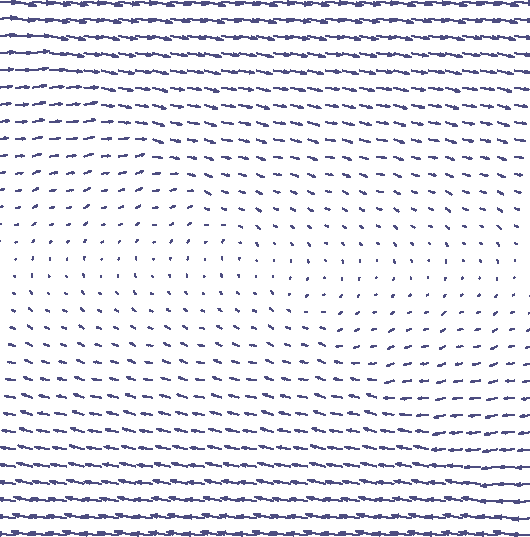
\includegraphics[width=\paperwidth,height=\paperheight]{figures/frontPage}};
\clearpage  
}  

\pgfdeclareimage[height=1.5cm]{titlepagelogo}{AAUgraphics/aau_logo_new} % placed on the title page
\titlegraphic{% is placed on the bottom of the title page
    \pgfuseimage{titlepagelogo}
    %  \hspace{1cm}\pgfuseimage{titlepagelogo2}
}

%Macro for 'where'-enviroment was improved by Andrea and Niels :-)

%-----------UNITS-------------------------------------------
\newcommand{\unit}[1]{&& \left[\si{#1}\right]}
%
%\newcommand{\unit}[1]{[\si{#1}]}            %<<| Use these if you want equations to be
%\newcommand{\eq}[2]{&&\si{#1} &= \si{#2}&&} %<<| centered.. .. will appear scrambled
%                                            %  | from one equation to the next though..
%                                            %  | and does not work with long equations.. :/
%
%-----------------------------------------------------------

%-----------WHERE ENVIRONMENT-------------------------------
\newenvironment{where}{\leavevmode{\parindent=1em\indent} Where:\\}{}
\newcommand{\va}[3]
{
  \begin{tabular}{p{20pt} p{40pt} p{290pt} l}
    & { $#1$ } & { #2 } & \ifthenelse{\isempty{ #3 }}  {}  {[{\si{#3}}]} \\
  \end{tabular}\\
}
%-----------------------------------------------------------

%-----------TikZ SETTINGS-----------------------------------
\tikzset{
  block/.style    = {draw, thick, rectangle,
                     minimum height = 2.1em,
                     minimum width = 1.7em},
  sum/.style      = {draw, circle, inner sep=3pt} %<--Adder
}
%-----------------------------------------------------------

%------------VECTORS----------------------------------------
\renewcommand{\vec}[1]{\boldsymbol{\mathbf{#1}}}

% the titlepage
%{\aauwavesbg%
\begin{frame}[plain,noframenumbering] % the plain option removes the header from the title page
  \titlepage
\end{frame}%}


%\definecolor{aaublue}{RGB}{33,26,82}% dark blue

\begin{frame}<handout:0>{Agenda}{}
    \begin{itemize}
        \item \textcolor{aaublue}{\textbf{Introduction}}
        \begin{itemize}
            \item[-] \textcolor{aaublue}{\textbf{Use Case}}
        \end{itemize}
        \item \textcolor{aaublue}{\textbf{System Description}}
        \item \textcolor{aaublue}{\textbf{Model}}
        \begin{itemize}
             \item[-] \textcolor{aaublue}{\textbf{Reference Frames}}
             \item[-] \textcolor{aaublue}{\textbf{Model Equations}}
             \item[-] \textcolor{aaublue}{\textbf{Model Verification}}
        \end{itemize}
        \item Control Approach
        \item Sensor Fusion
        \item Inner Controller
        \item Outer Controller
        \item Results
        \item Conclusion
    \end{itemize}
\end{frame}
%%%%%%%%%%%%%%%%%
\section{Introduction}

\begin{frame}{Introduction}{}
    \begin{figure}[H]
        \centering
        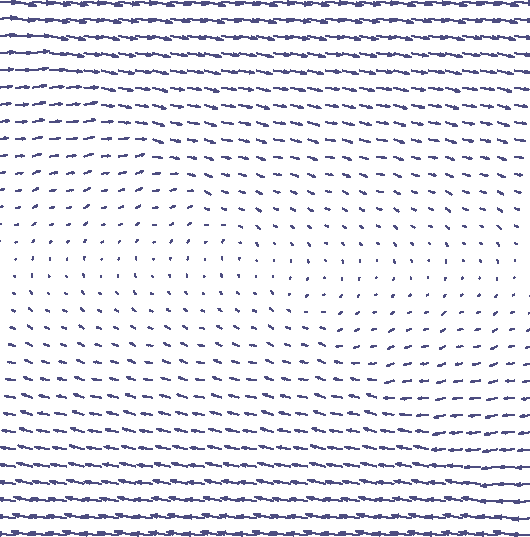
\includegraphics[width=.6\linewidth]{figures/frontpage}
    \end{figure}
    \begin{itemize}
         \item Environmental monitoring
         \item Marine biological research
         \item Bathymetric measurements
         \item Control theory for an ASV
    \end{itemize}
\end{frame}

\begin{frame}{Introduction}{Use Case}
    \begin{figure}[H]
        \centering
        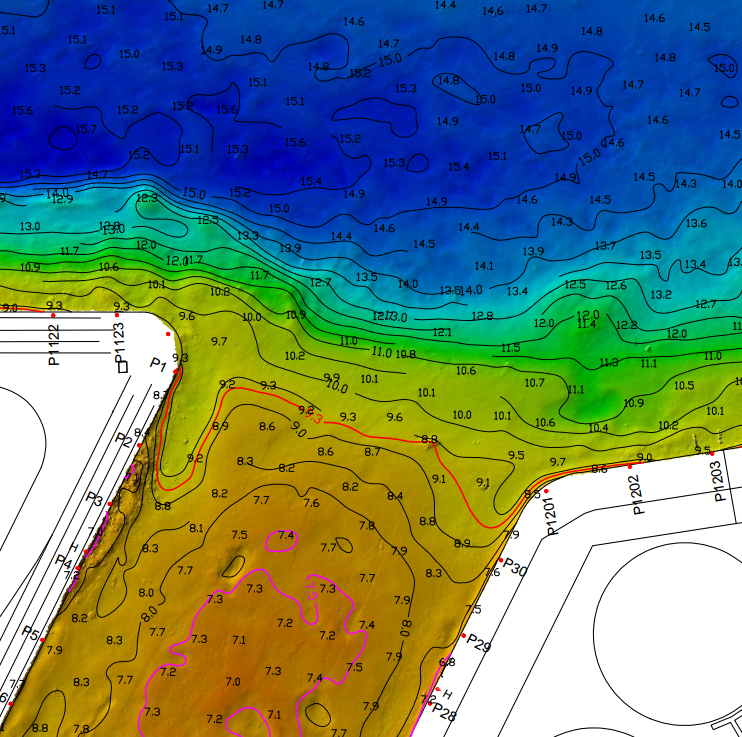
\includegraphics[width=.4\linewidth]{figures/smallDebthMapAalborg}
    \end{figure}
    \begin{itemize}
        \item Depth map used by Port of Aalborg 
        \item Problem: No recent knowledge of depths of the port
        \item Solution: Automate smaller unmanned vessel
    \end{itemize}
\end{frame}

\section{System Description}
\begin{frame}{System Description}{}
    \begin{minipage}{0.47\linewidth}
    \begin{figure}[H]
        \centering
        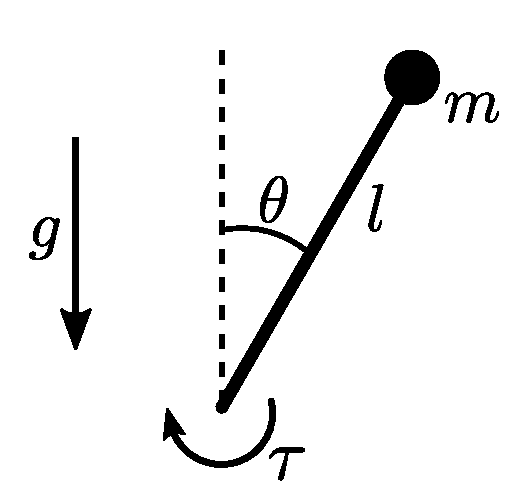
\includegraphics[width=1\linewidth]{figures/system}
    \end{figure}        
    \end{minipage}\hfill      
    \begin{minipage}{0.49\linewidth}
    \begin{figure}[H]
        \centering
        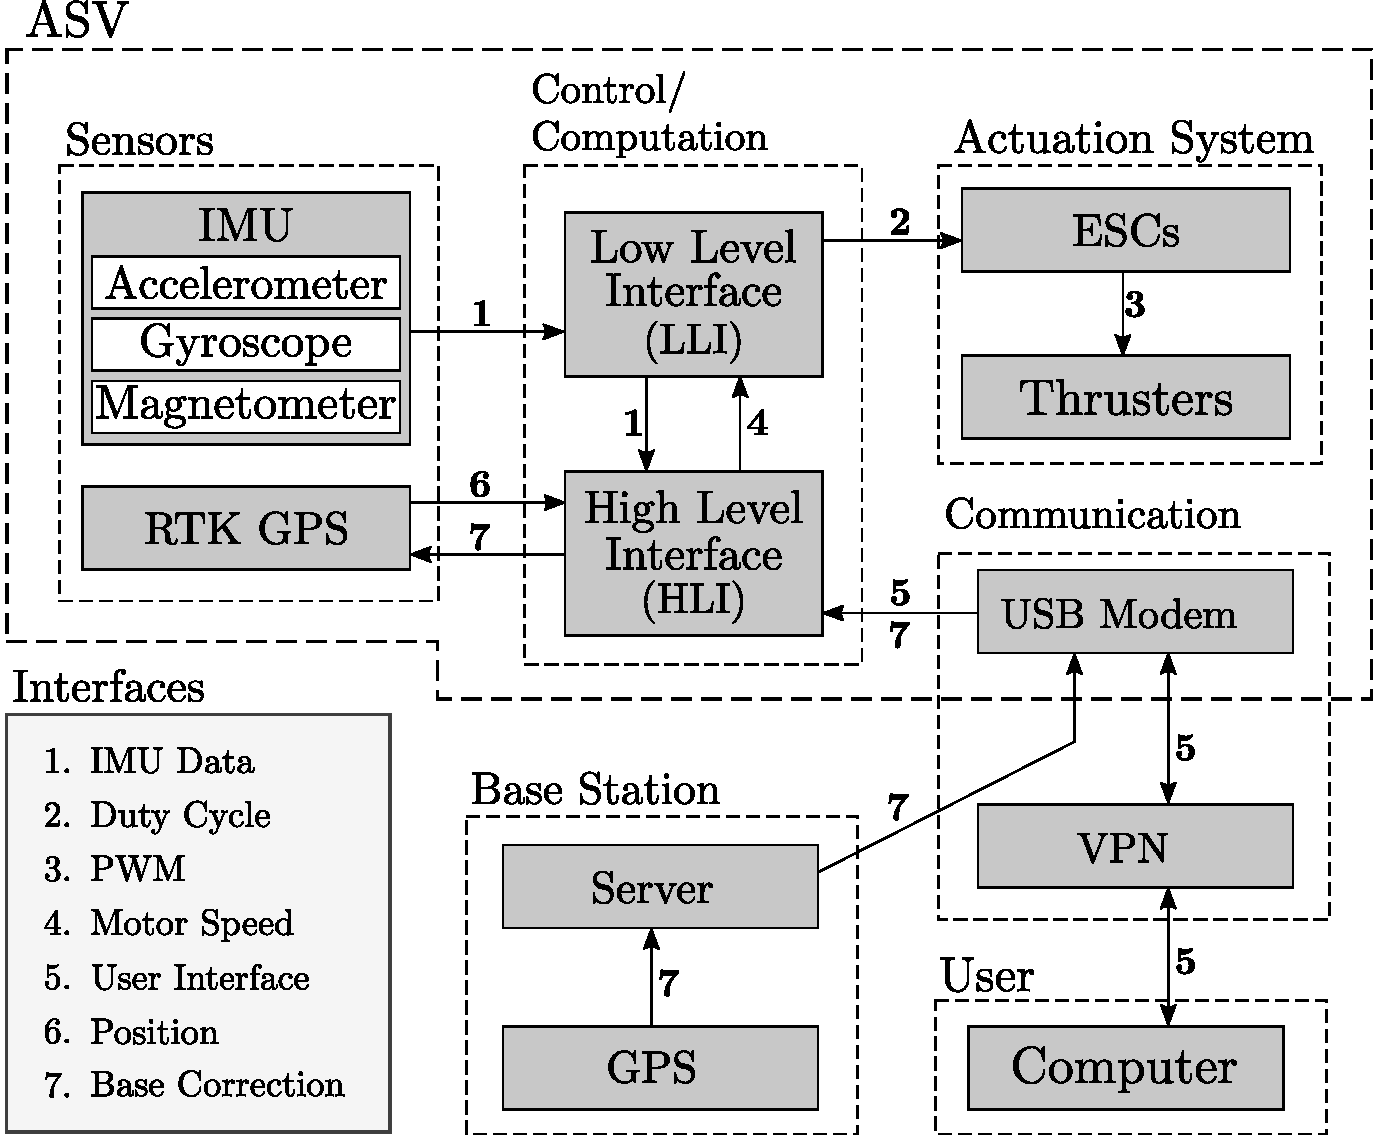
\includegraphics[width=1\linewidth]{figures/systemDiagram5}
    \end{figure}                
    \end{minipage}\hfill \\
\end{frame}

\begin{frame}{System Description}{RTK GPS}
    \begin{figure}[H]
        \centering
        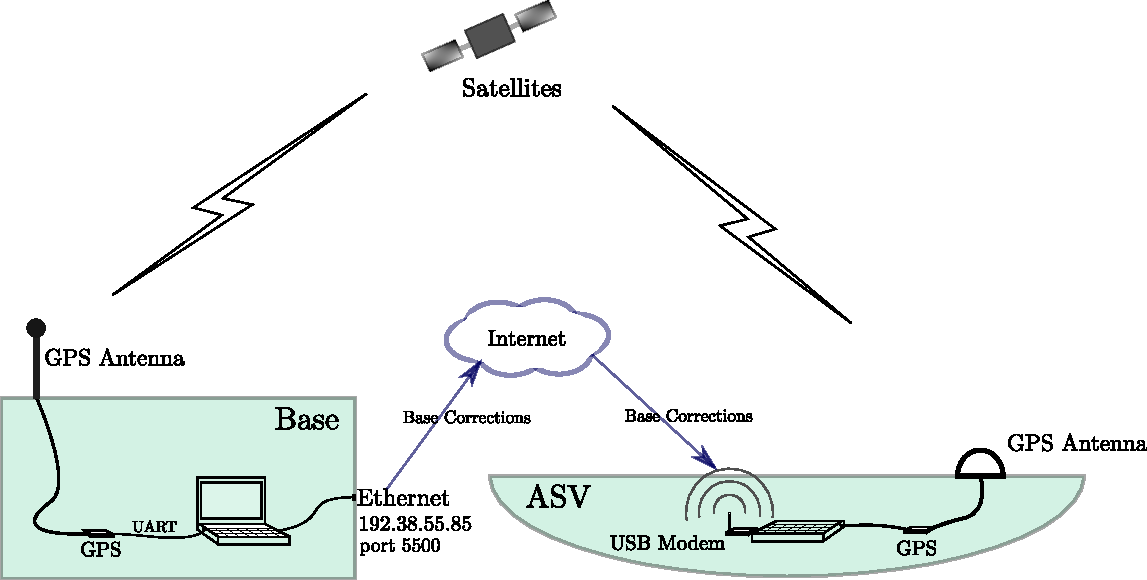
\includegraphics[width=0.7\linewidth]{figures/comunicationSetup}
    \end{figure}        

\end{frame}

%%%%%%%%%%%%%%%%
\section{Model}

%\subsection{Reference Frames}
\begin{frame}{Model}{Reference Frames}
    \begin{figure}[H]
        \centering
        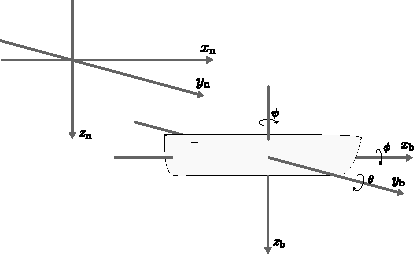
\includegraphics[width=0.7\linewidth]{figures/boat3D}
    \end{figure}
    \begin{itemize}
        \item Inertial Frame (NED)
        \item Body Frame
    \end{itemize}
\end{frame}

%\subsection{Model Dynamics}
\begin{frame}{Model}{Model Dynamics}
    \begin{minipage}{0.5\linewidth}
        \begin{figure}[H]
            \centering
            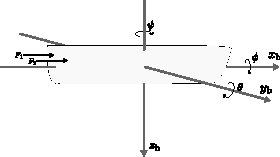
\includegraphics[width=0.8\linewidth]{figures/boat3DForces}
        \end{figure}
        \begin{figure}[H]
            \centering
            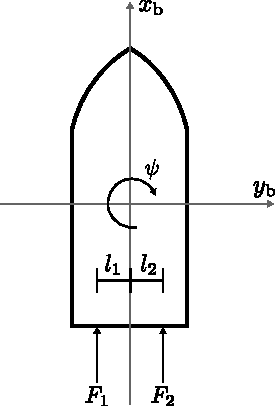
\includegraphics[width=0.4\linewidth]{figures/boat2D}
        \end{figure}         
    \end{minipage}\hfill      
    \begin{minipage}{0.5\linewidth}
        \begin{itemize}
            \item Rigid Body Dynamics
            \begin{flalign}
                \sum F&=m \ddot{x} \nonumber \\
                \sum \tau&=I \ddot{\theta} \nonumber
            \end{flalign}
            \item Hydrostatics
            \begin{itemize}
                \item[-] Buoyancy Force
            \end{itemize}
            \item Hydrodynamics
            \begin{itemize}
                \item[-] Viscous Damping
            \end{itemize}
        \end{itemize}              
    \end{minipage}\hfill \\
\end{frame}

% %\subsection{Rigid Body Dynamics}
% \begin{frame}{Model}{Rigid Body Dynamics}
%     \begin{minipage}{0.65\linewidth}
%         \begin{figure}[H]
%             \centering
%             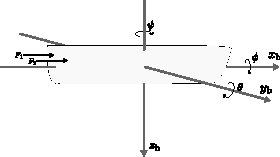
\includegraphics[width=1\linewidth]{figures/boat3DForces}
%         \end{figure}        
%     \end{minipage}\hfill      
%     \begin{minipage}{0.3\linewidth}
%         \begin{figure}[H]
%             \centering
%             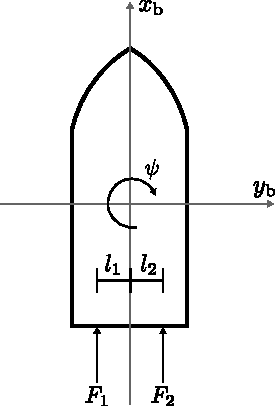
\includegraphics[width=0.7\linewidth]{figures/boat2D}
%         \end{figure}                
%     \end{minipage}\hfill \\
%     \begin{flalign}
%         \sum F&=m \ddot{x} \nonumber \\
%         \sum \tau&=I \ddot{\theta} \nonumber
%     \end{flalign}
% \end{frame}

% %\subsection{Hydrostatics}
% \begin{frame}{Model}{Hydrostatics}
%     \begin{minipage}{0.65\linewidth}
%         \begin{figure}[H]
%             \centering
%             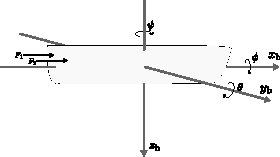
\includegraphics[width=1\linewidth]{figures/boat3DForces}
%         \end{figure}        
%     \end{minipage}\hfill      
%     \begin{minipage}{0.3\linewidth}
%         \begin{figure}[H]
%             \centering
%             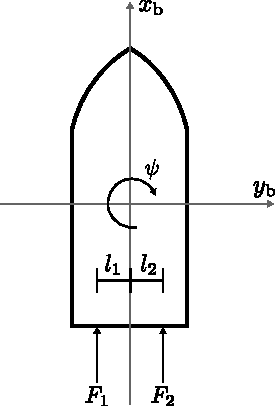
\includegraphics[width=0.7\linewidth]{figures/boat2D}
%         \end{figure}                
%     \end{minipage}\hfill \\
%     \begin{itemize}
%         \item Buoyancy Force
%     \end{itemize}
% \end{frame}

% %\subsection{Hydrodynamics}
% \begin{frame}{Model}{Hydrodynamics}
%     \begin{minipage}{0.65\linewidth}
%         \begin{figure}[H]
%             \centering
%             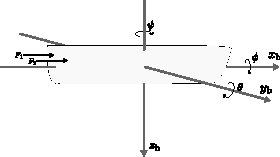
\includegraphics[width=1\linewidth]{figures/boat3DForces}
%         \end{figure}        
%     \end{minipage}\hfill      
%     \begin{minipage}{0.3\linewidth}
%         \begin{figure}[H]
%             \centering
%             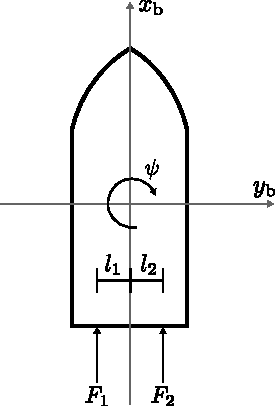
\includegraphics[width=0.7\linewidth]{figures/boat2D}
%         \end{figure}                
%     \end{minipage}\hfill \\
%     \begin{itemize}
%         \item Added mass
%         \item Viscous Damping
%     \end{itemize}
% \end{frame}

%\subsection{Model Equations}
\begin{frame}{Model}{Model Equations}
    \begin{minipage}{0.5\linewidth}
        \begin{figure}[H]
            \centering
            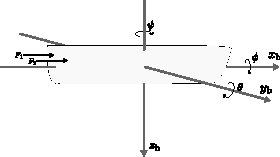
\includegraphics[width=0.8\linewidth]{figures/boat3DForces}
          \end{figure}
          \begin{figure}[H]
              \centering
              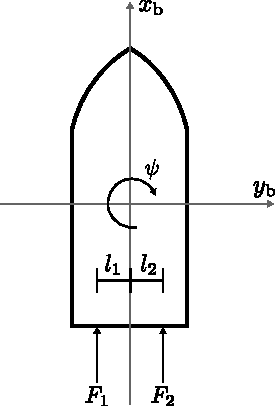
\includegraphics[width=0.4\linewidth]{figures/boat2D}
          \end{figure}         
      \end{minipage}\hfill      
    \begin{minipage}{0.5\linewidth}
        \begin{flalign}
            m \ddot{x}_\mathrm{b} &=  F_\mathrm{1} + F_\mathrm{2}  - d_{\dot{x}_\mathrm{b}} \dot{x}_\mathrm{b} + F_{x_\mathrm{b}}  \nonumber \\
            m \ddot{y}_\mathrm{b} &=  -d_{\dot{y}_\mathrm{b}} \dot{y_\mathrm{b}} + F_{y_\mathrm{b}}  \nonumber \\
            m \ddot{z}_\mathrm{b} &=  -d_{\dot{z}_\mathrm{b}}\dot{z_\mathrm{b}} + F_{z_\mathrm{b}}  \nonumber \\
            I_\mathrm{x}\ddot{\phi} &= -d_{\dot{\phi}} \dot{\phi} + T_\mathrm{\phi}   \nonumber \\
            I_\mathrm{y}\ddot{\theta} &= -d_{\dot{\theta}} \dot{\theta} + T_\mathrm{\theta}   \nonumber \\
            I_\mathrm{z}\ddot{\psi} &= F_\mathrm{1}l_\mathrm{1} - F_\mathrm{2} l_\mathrm{2} - d_{\dot{\psi}} \dot{\psi}  \nonumber
        \end{flalign}              
    \end{minipage}\hfill \\
\end{frame}

%\subsection{Model Equations}
\begin{frame}{Model}{Linearized Model Equations}
    \begin{minipage}{0.5\linewidth}
        \begin{figure}[H]
            \centering
            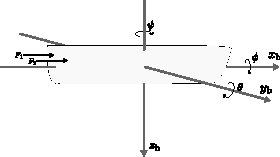
\includegraphics[width=0.8\linewidth]{figures/boat3DForces}
          \end{figure}
          \begin{figure}[H]
              \centering
              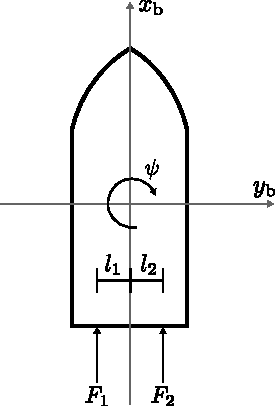
\includegraphics[width=0.4\linewidth]{figures/boat2D}
          \end{figure}         
      \end{minipage}\hfill      
    \begin{minipage}{0.5\linewidth}
        \begin{flalign}
            m \ddot{x}_\mathrm{b} &=  F_\mathrm{1} + F_\mathrm{2}  - d_{\dot{x}_\mathrm{b}} \dot{x}_\mathrm{b} \nonumber \\
            m \ddot{y}_\mathrm{b} &=  -d_{\dot{y}_\mathrm{b}} \dot{y_\mathrm{b}} \nonumber \\
            m \ddot{z}_\mathrm{b} &=  -d_{\dot{z}_\mathrm{b}}\dot{z_\mathrm{b}} -\rho g A_\mathrm{wp} \tilde{z}_\mathrm{n} \nonumber  \\
            I_\mathrm{x}\ddot{\phi} &= -d_{\dot{\phi}} \dot{\phi} - \rho g V \overline{GM_{T}}\cdot \phi \nonumber \\
            I_\mathrm{y}\ddot{\theta} &= -d_{\dot{\theta}} \dot{\theta} - \rho g V \overline{GM_{L}}\cdot \theta \nonumber \\
            I_\mathrm{z}\ddot{\psi} &= F_\mathrm{1}l_\mathrm{1} - F_\mathrm{2} l_\mathrm{2} - d_{\dot{\psi}} \dot{\psi} \nonumber
        \end{flalign}              
    \end{minipage}\hfill \\
\end{frame}

% %\subsection{Model Equations 2}
% \begin{frame}{Model}{Model Equations 2}
%     \begin{minipage}{0.3\linewidth}
%         \begin{figure}[H]
%             \centering
%             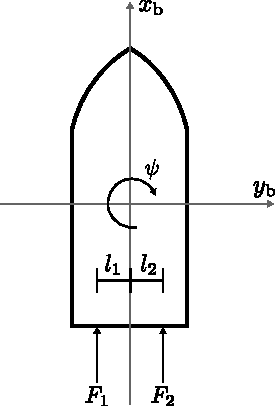
\includegraphics[width=1\linewidth]{figures/boat2D}
%         \end{figure}        
%     \end{minipage}\hfill      
%     \begin{minipage}{0.65\linewidth}
%         \begin{flalign}
%             m \ddot{x}_\mathrm{b} &=  F_\mathrm{1} + F_\mathrm{2}  - d_{\dot{x}_\mathrm{b}} \dot{x}_\mathrm{b} + F_{x_\mathrm{b}}  \nonumber \\
%             m \ddot{y}_\mathrm{b} &=  -d_{\dot{y}_\mathrm{b}} \dot{y_\mathrm{b}} + F_{y_\mathrm{b}}  \nonumber \\
%             m \ddot{z}_\mathrm{b} &=  -d_{\dot{z}_\mathrm{b}}\dot{z_\mathrm{b}} + F_{z_\mathrm{b}}  \nonumber \\
%             I_\mathrm{x}\ddot{\phi} &= -d_{\dot{\phi}} \dot{\phi} + T_\mathrm{\phi}   \nonumber \\
%             I_\mathrm{y}\ddot{\theta} &= -d_{\dot{\theta}} \dot{\theta} + T_\mathrm{\theta}   \nonumber \\
%             I_\mathrm{z}\ddot{\psi} &= F_\mathrm{1}l_\mathrm{1} - F_\mathrm{2} l_\mathrm{2} - d_{\dot{\psi}} \dot{\psi}  \nonumber
%         \end{flalign}              
%     \end{minipage}\hfill \\
% \end{frame}

%\subsection{Model Verification}
\begin{frame}{Model}{Model Verification}
    \begin{itemize}
        \item Verified model
    \end{itemize}
    \begin{minipage}{0.45\linewidth}
        \begin{figure}[H]
            \centering
            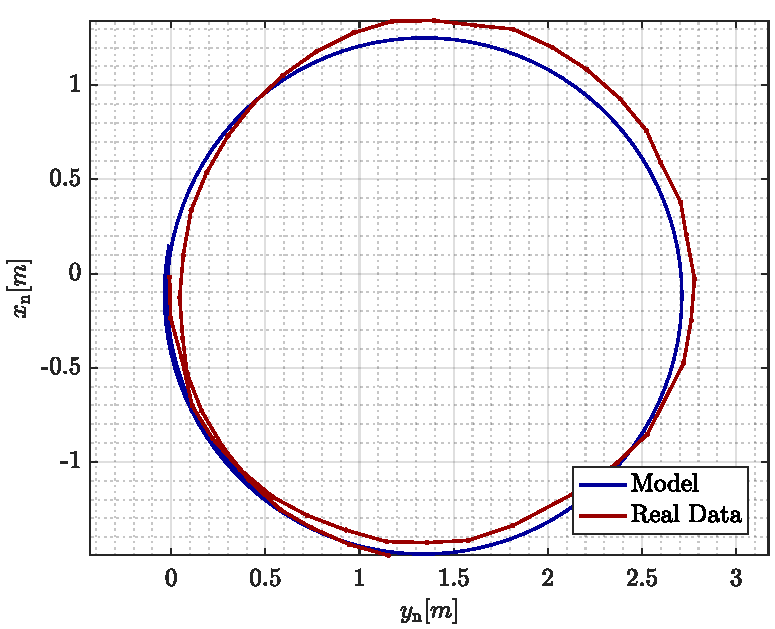
\includegraphics[width=1\linewidth]{figures/turn}
        \end{figure}        
    \end{minipage}\hfill      
    \begin{minipage}{0.45\linewidth}
        \begin{figure}[H]
            \centering
            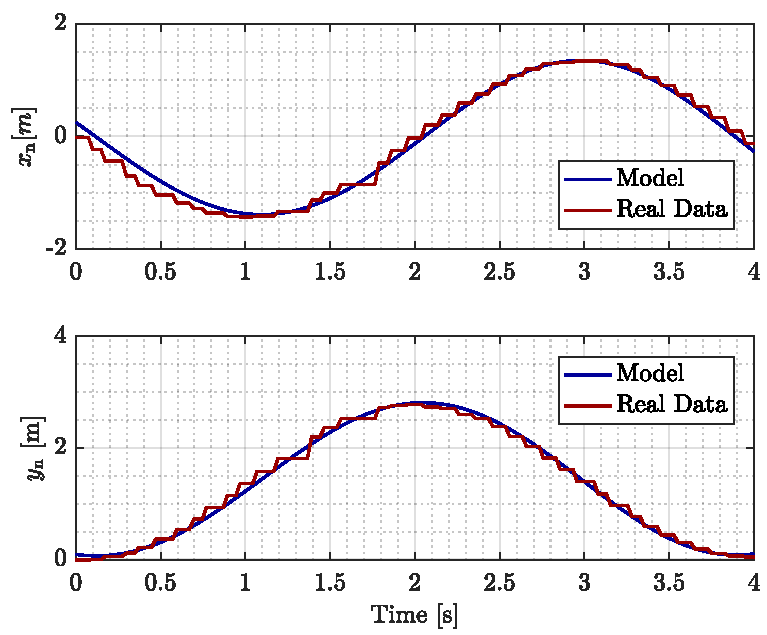
\includegraphics[width=1\linewidth]{figures/turn_time}
        \end{figure}                
    \end{minipage}\hfill \\
\end{frame}








%\definecolor{aaublue}{RGB}{33,26,82}% dark blue

\begin{frame}<handout:0>{Agenda}{}
    \begin{itemize}
        \item Introduction
        \item System Description
        \item Model
        \item \textcolor{aaublue}{\textbf{Control Approach}}
        \item \textcolor{aaublue}{\textbf{Sensor Fusion}}
        \begin{itemize}
            \item[-] \textcolor{aaublue}{\textbf{Attitude Kalman Filter}}
            \item[-] \textcolor{aaublue}{\textbf{Position Kalman Filter}}
        \end{itemize}
        \item Inner Controller
        \item Outer Controller
        \item Results
        \item Conclusion
    \end{itemize}
\end{frame}
%%%%%%%%%%%%%%%%%
\section{Control Approach}

\begin{frame}{Control Approach}{}
    \begin{figure}[H]
        \centering
        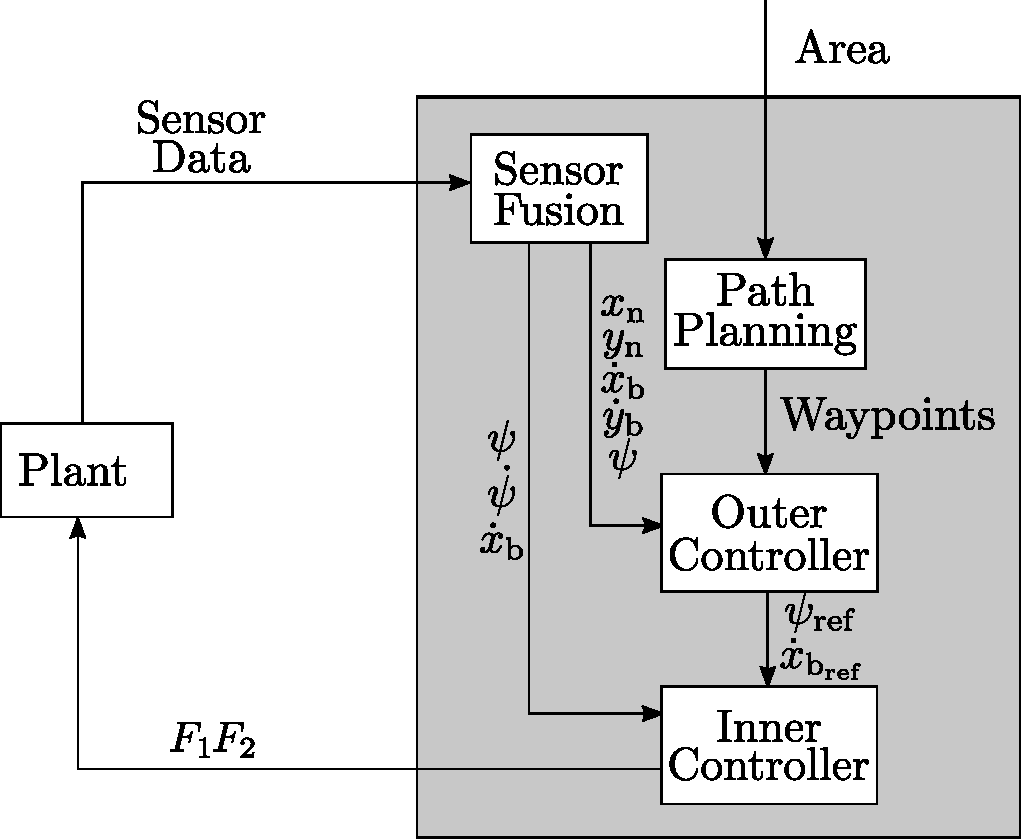
\includegraphics[width=.6\linewidth]{figures/controllerDiagram2}
    \end{figure}
\end{frame}

%%%%%%%%%%%%%%%%
\section{Sensor Fusion}

\begin{frame}{Sensor Fusion}{Structure}
	\begin{itemize}

		\item Fuses GPS and IMU data
		\item Achieved using a Kalman filter
		\item Sensor fusion contains
			\begin{itemize}
		\item Attitude
		\item Position
			\end{itemize}
	\end{itemize}

\end{frame}
\begin{frame}{Sensor Fusion}{Signal Model}
	\begin{gather*}
    \vec{x}_\mathrm{KF}(k+1) = \vec{A}_\mathrm{KF}\vec{x}_\mathrm{KF}(k) + \vec{B}_\mathrm{KF} \vec{u}(k) + \vec{w}_\mathrm{KF}(k)  \nonumber \\
    \vec{y}_\mathrm{KF}(k+1) = \vec{C}_\mathrm{KF} \vec{x}_\mathrm{KF}(k+1) + \vec{v}_\mathrm{KF}(k+1)  \nonumber
    \end{gather*}
    \begin{figure}[H]
        \centering
        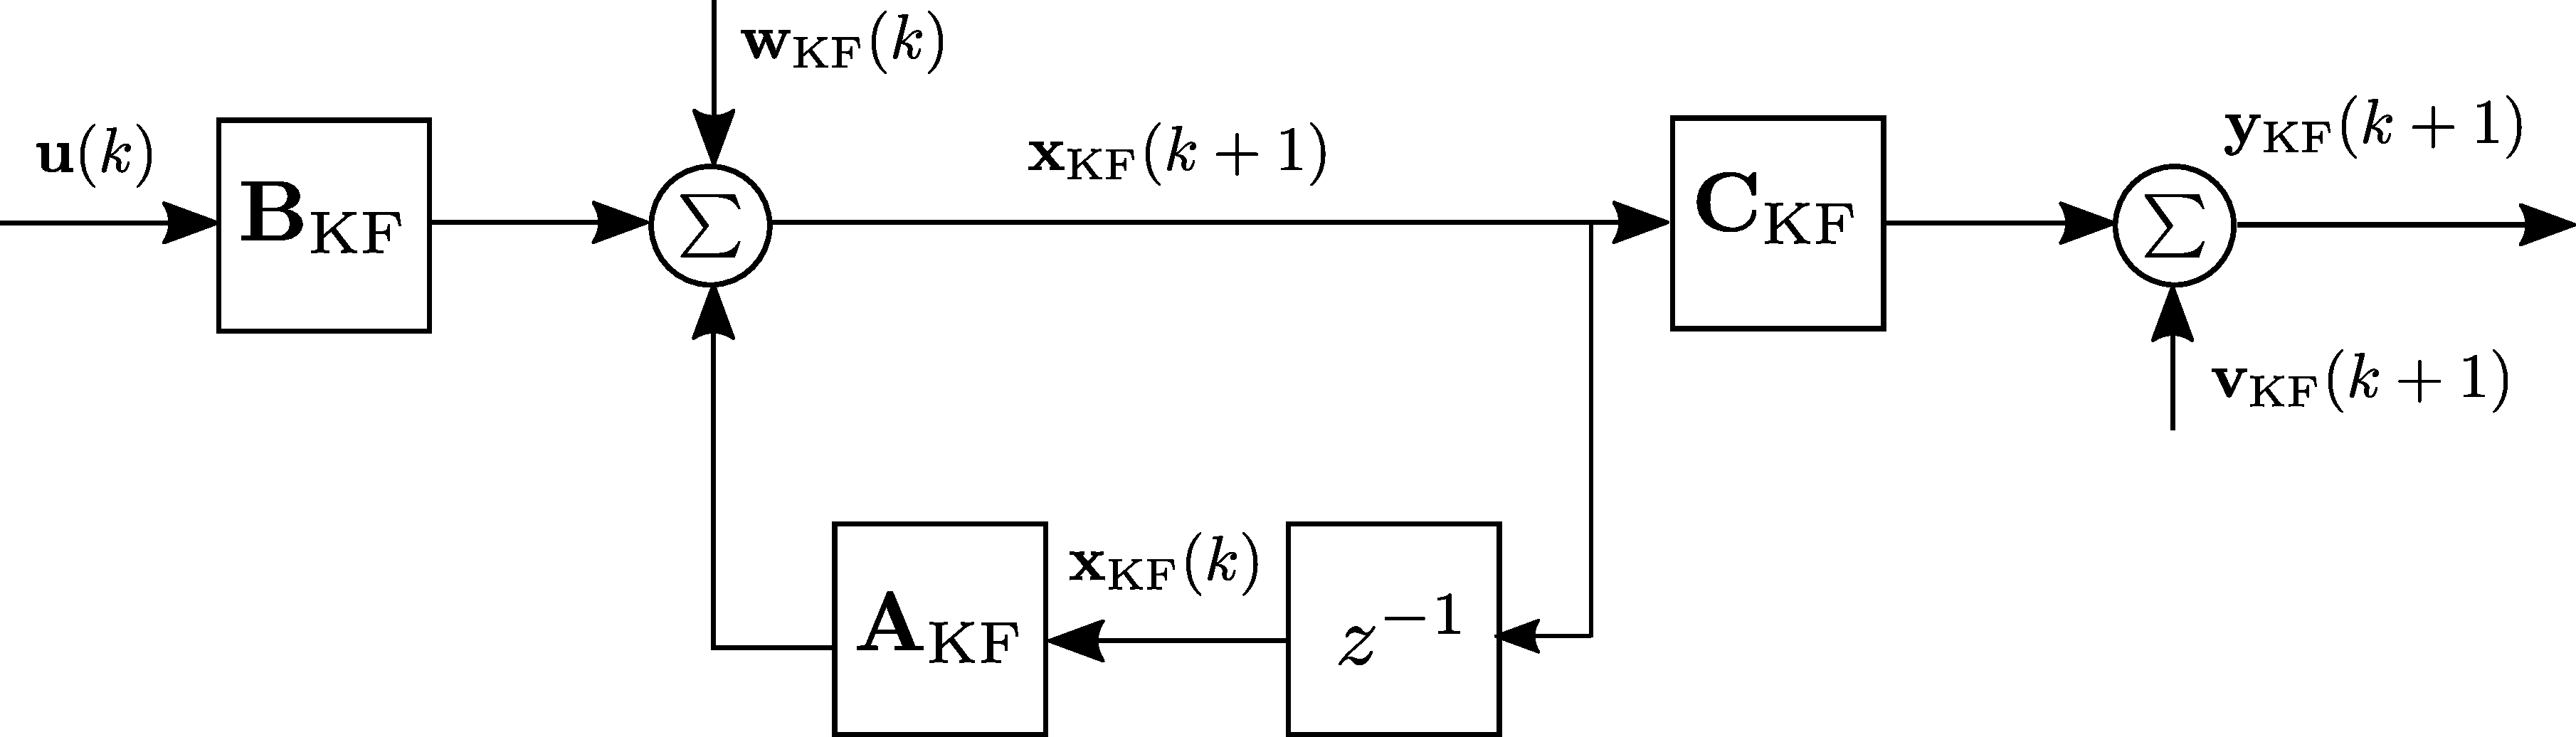
\includegraphics[width=.7\linewidth]{figures/signalModel}
    \end{figure}
	\begin{itemize}
		\item w(k) and v(k) are assumed white Gaussian
		\item Matrices $\vec{Q}_\mathrm{KF}$ and $\vec{R}_\mathrm{KF}$ are the respective covariance matrices
	\end{itemize}

\end{frame}

\begin{frame}{Sensor Fusion}{Signal Model - State and Measurement Vectors}
    \begin{flalign}
        \vec{u} = 
        \begin{bmatrix}
        F_1 & F_2
        \end{bmatrix}^\mathrm{T}  \nonumber
    \end{flalign}
\begin{itemize}
    \item Attitude
    \begin{gather*}
        \vec{x}_\mathrm{att} = 
        \begin{bmatrix}
        \phi & \theta & \psi & \dot{\phi} & \dot{\theta} & \dot{\psi} & \ddot{\phi} & \ddot{\theta} & \ddot{\psi}
        \end{bmatrix}^\mathrm{T}  \nonumber \\
        \vec{y}_\mathrm{att} =
        \begin{bmatrix}
        \phi_\mathrm{acc} & \theta_\mathrm{acc} & \psi_\mathrm{mag} & \dot{\phi}_\mathrm{gyro} & \dot{\theta}_\mathrm{gyro} & \dot{\psi}_\mathrm{gyro}
        \end{bmatrix}^\mathrm{T} \nonumber
    \end{gather*}
	\item Position
    \begin{gather*}
        \vec{x}_\mathrm{pos} =
        \begin{bmatrix}
        x_\mathrm{n} & y_\mathrm{n} & \dot{x}_\mathrm{b} & \dot{y}_\mathrm{b} & \ddot{x}_\mathrm{b} & \ddot{y}_\mathrm{b}
        \end{bmatrix}^\mathrm{T} \nonumber \\
        \vec{y}_\mathrm{pos} =
        \begin{bmatrix}
        x_\mathrm{n,GPS} & y_\mathrm{n,GPS} & \ddot{x}_\mathrm{b,acc} & \ddot{y}_\mathrm{b,acc}
        \end{bmatrix}^\mathrm{T} \nonumber
    \end{gather*}
    \end{itemize}
\end{frame}


\begin{frame}{Sensor Fusion}{Kalman Filter}

	\begin{itemize}
		\item Step 0: Initialization
        \begin{flalign}
        	\hat{\vec{x}}_\mathrm{KF}(0|0) &= \vec{0} \nonumber\\
        	\vec{P}_\mathrm{KF}(0|0) &= \vec{Q}_\mathrm{KF}\nonumber
        \end{flalign}
		\item Step 1: Prediction
		\item Step 2: Update
   	\end{itemize}
\end{frame}


\begin{frame}{Sensor Fusion}{Kalman Filter}
	\begin{itemize}
		\item Step 0: Initialization
		\item Step 1: Prediction
        {\footnotesize
        \begin{flalign}
            \hat{\vec{x}}_\mathrm{KF}(k+1|k) &= \vec{A}_\mathrm{KF} \hat{\vec{x}}_\mathrm{KF}(k|k) + \vec{B}_\mathrm{KF} \vec{u}(k) \nonumber\\
            \vec{P}(k+1|k) &= \vec{A}_\mathrm{KF} \vec{P}(k|k) \vec{A}_\mathrm{KF}^\mathrm{T} + \vec{Q}_\mathrm{KF} \nonumber
        \end{flalign}}
	 	\item Step 2: Update
         {\footnotesize
        \begin{gather*}
            \hat{\vec{x}}_\mathrm{KF}(k+1|k+1) = \hat{\vec{x}}_\mathrm{KF}(k+1|k) +  \vec{K}(k+1) \left[ \vec{y}_\mathrm{KF}(k+1) - \vec{C}_\mathrm{KF}  \hat{\vec{x}}_\mathrm{KF}(k+1|k) \right] \nonumber\\
            \vec{P}(k+1|k+1) = \left[ \vec{I} - \vec{K}(k+1) \vec{C}_\mathrm{KF}^\mathrm{T} \right] \vec{P}(k+1|k)\nonumber
        \end{gather*}}
	\end{itemize}
\end{frame}

\begin{frame}{Sensor Fusion}{Kalman Filter}
    \begin{figure}[H]
        \centering
        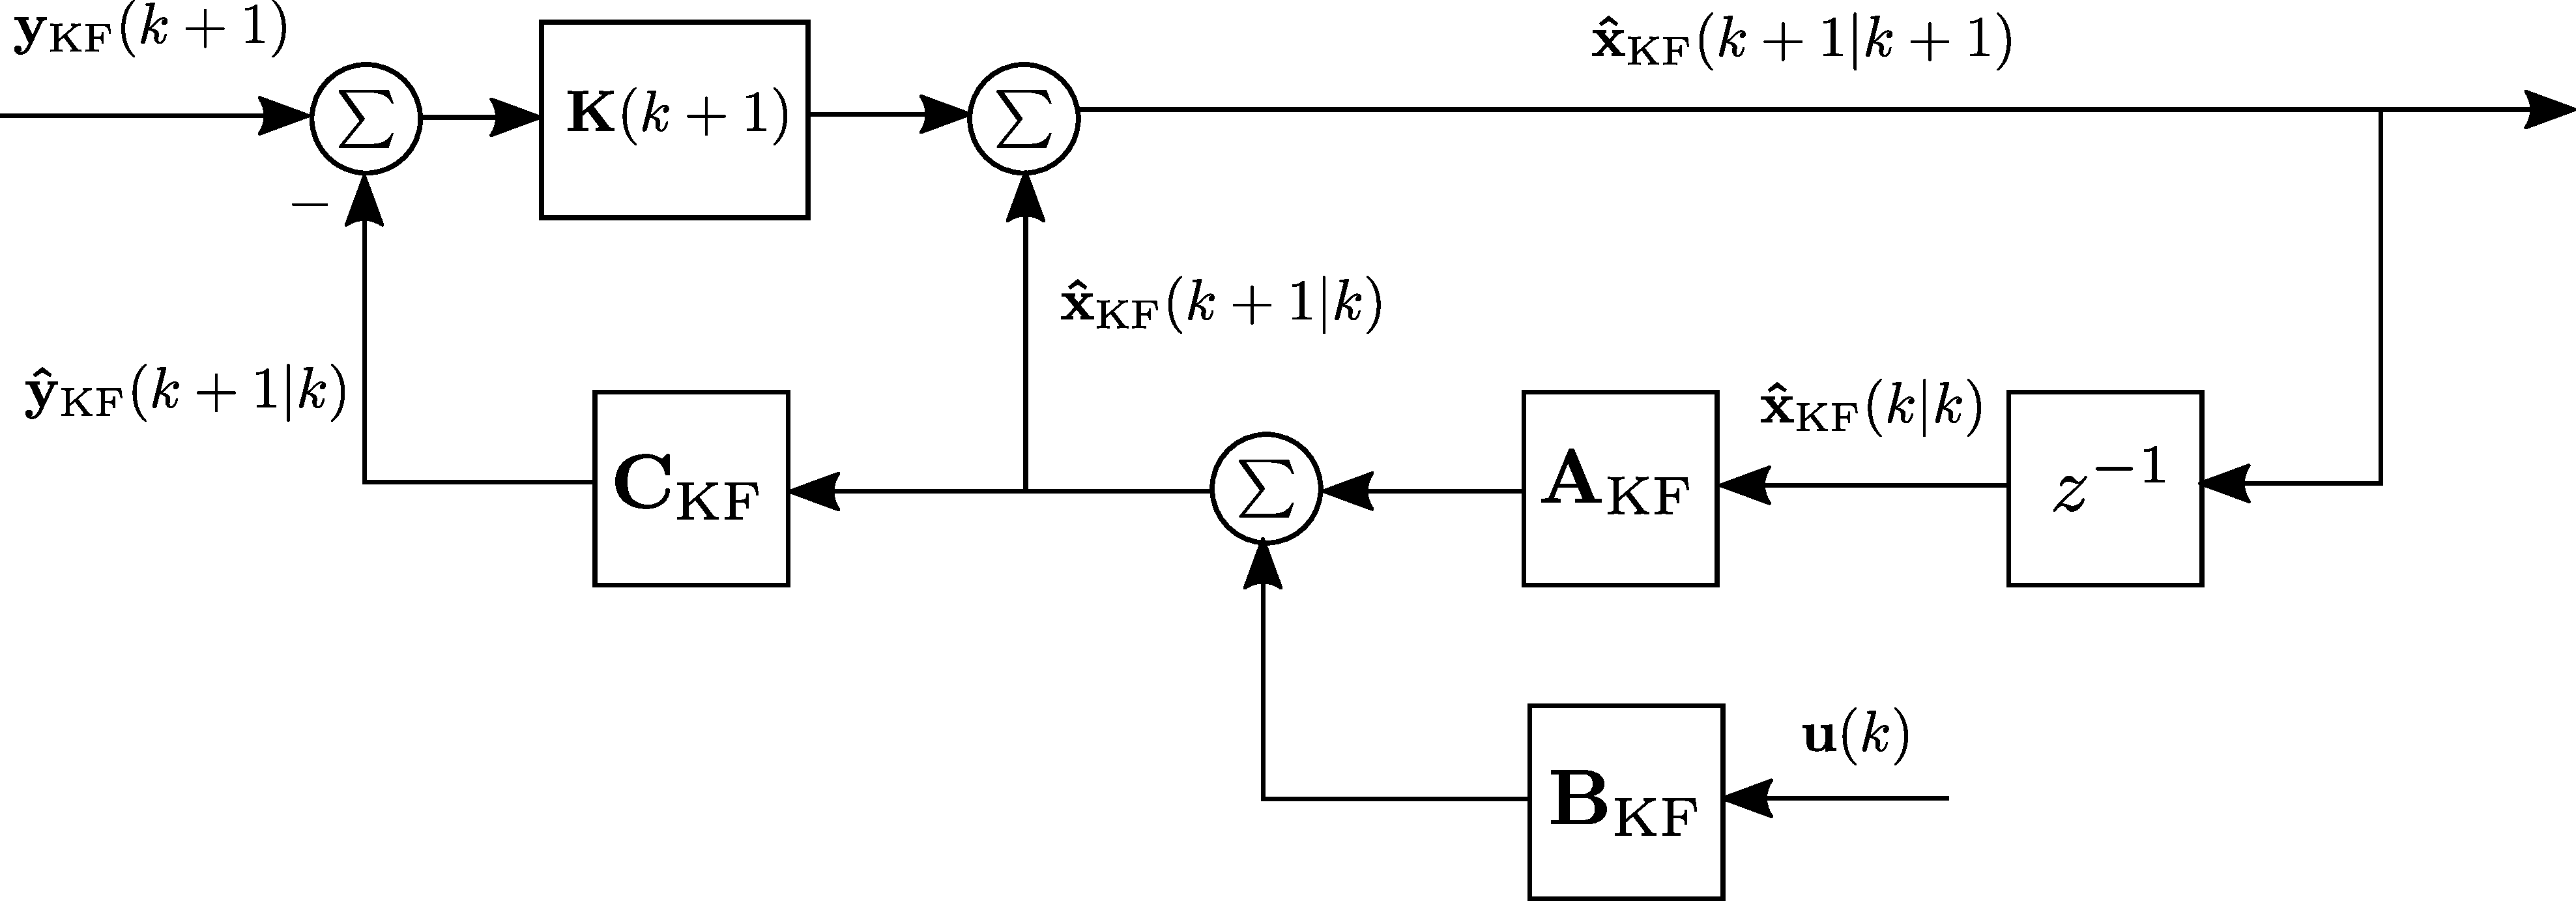
\includegraphics[width=.95\linewidth]{figures/kalmanFilter}
    \end{figure}
\end{frame}

\begin{frame}{Sensor Fusion}{Attitude Kalman Filter}
    \begin{figure}[H]
        \centering
        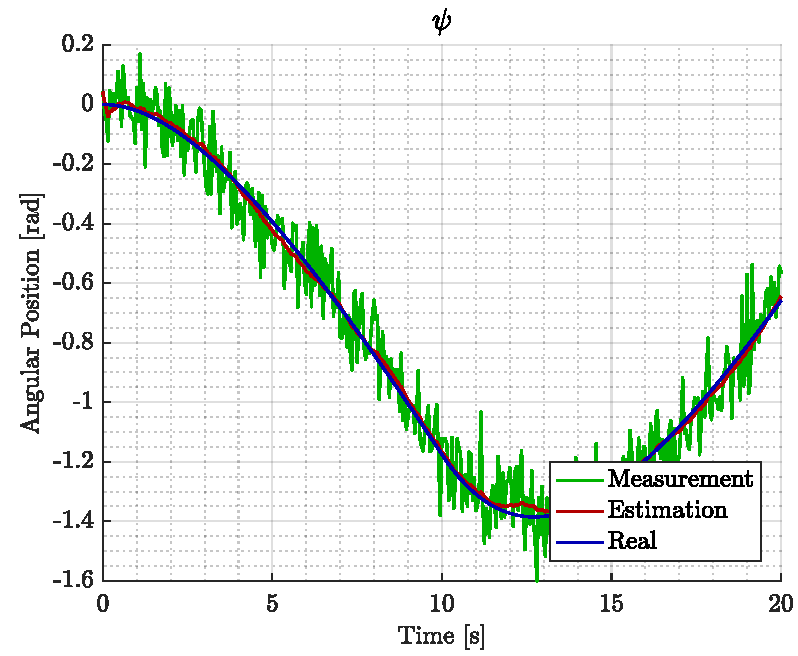
\includegraphics[width=0.6\linewidth]{figures/sim_yaw}
    \end{figure}
\end{frame}

\begin{frame}{Sensor Fusion}{Position Kalman Filter}
    \begin{minipage}{0.45\linewidth}
        \begin{figure}[H]
            \centering
            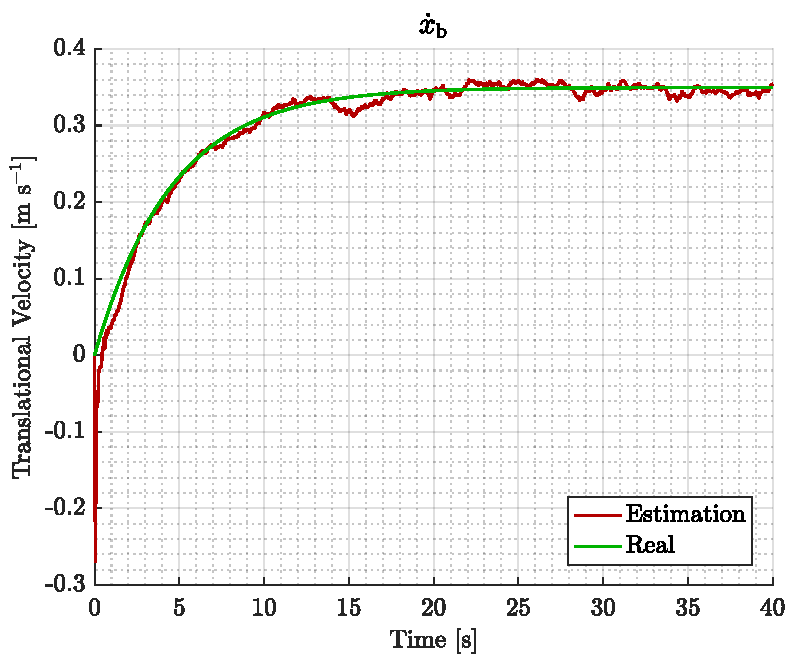
\includegraphics[width=1\linewidth]{figures/sim_xbdot}
        \end{figure}        
    \end{minipage}\hfill      
    \begin{minipage}{0.45\linewidth}
        \begin{figure}[H]
            \centering
            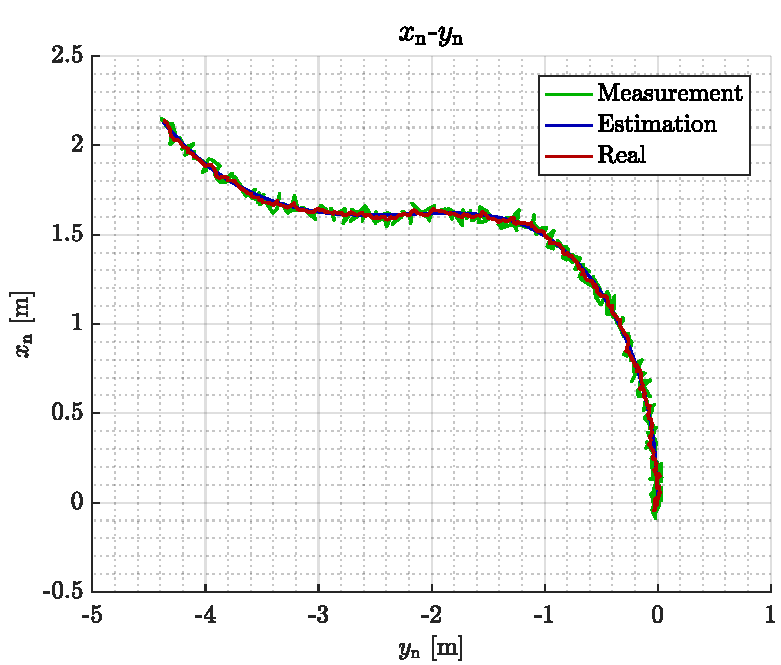
\includegraphics[width=1\linewidth]{figures/sim_xnyn}
        \end{figure}                
    \end{minipage}\hfill \\
\end{frame}



%\definecolor{aaublue}{RGB}{33,26,82}% dark blue

\begin{frame}<handout:0>{Agenda}{}
    \begin{itemize}
        \item Introduction
        \item System Description
        \item Model
        \item Control Approach
        \item Sensor Fusion
        \item \textcolor{aaublue}{\textbf{Inner Controller}}
        \begin{itemize}
            \item[-] \textcolor{aaublue}{\textbf{$\mathcal{H}_\infty$ Controller Design}}
            \item[-] Linear Quadratic Regulator Design
            \item[-] Comparison of the Controllers
        \end{itemize}
        \item Outer Controller
        \item Results
        \item Conclusion
    \end{itemize}
\end{frame}
%%%%%%%%%%%%%%%%%
\section{Inner Controller}

\begin{frame}{Inner Controller}{}
    \uncover<1-3>{
    \begin{figure}[H]
        \centering
        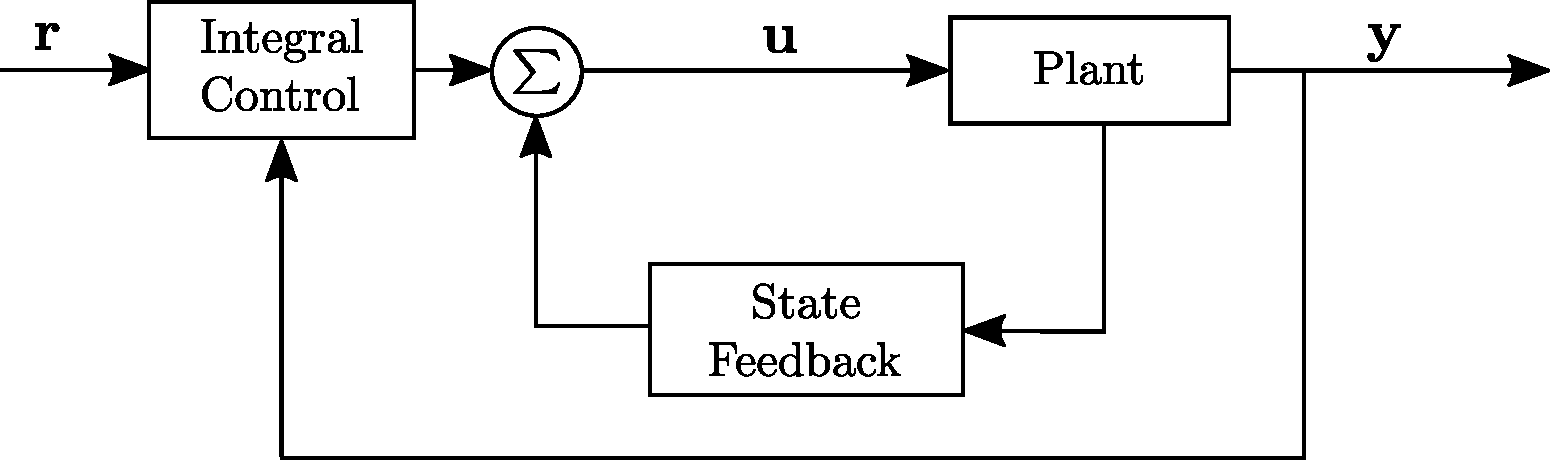
\includegraphics[width=0.6\linewidth]{figures/ControlDiagram}
    \end{figure}}
    \uncover<2-3>{
        \vspace{-0.3cm}
        \begin{itemize}
            \item Plant
        \end{itemize}
    \begin{figure}[H]
        \centering
        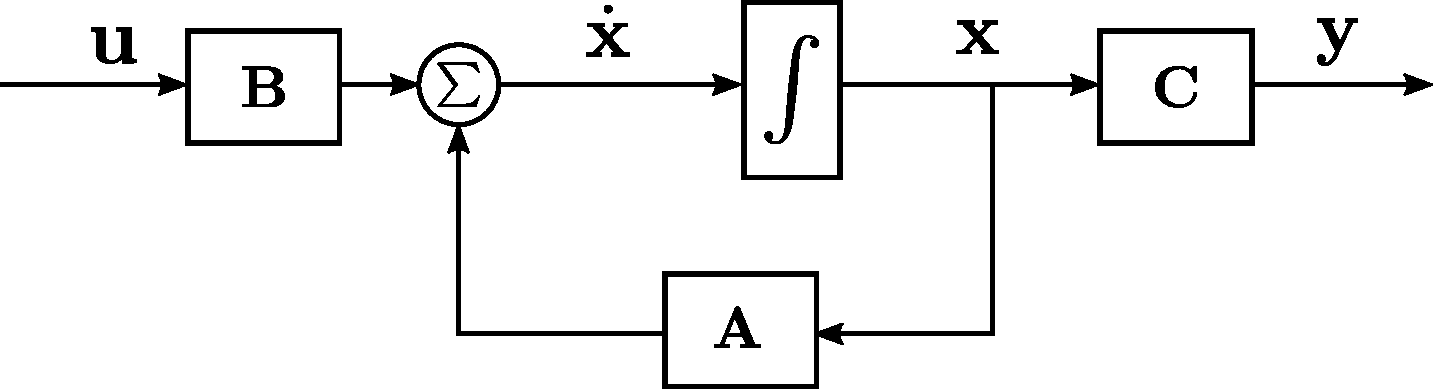
\includegraphics[width=0.45\linewidth]{figures/PlantSS}
    \end{figure}}
    \uncover<3>{
        \vspace{-0.3cm}
    \begin{itemize}
        \item Approaches
        \begin{itemize}
            \item $\mathcal{H}_\infty$ Controller
            \item Linear Quadratic Regulator
        \end{itemize}
    \end{itemize}}
\end{frame}

\begin{frame}{Inner Controller}{$\mathcal{H}_\infty$ Controller Design}
    \begin{itemize}
        \item Suboptimal $\mathcal{H}_\infty$ controller
    \end{itemize}
    \vspace{0.2cm}
    \begin{center}
        Find an internally stabilizing controller that provides a closed loop $\mathcal{H}_\infty$ norm less than some bound $\gamma$
    \end{center}
\end{frame}

\begin{frame}{Inner Controller}{$\mathcal{H}_\infty$ Controller Design}
    \begin{itemize}
        \item System structure
    \end{itemize}
    \begin{figure}[H]
        \centering
        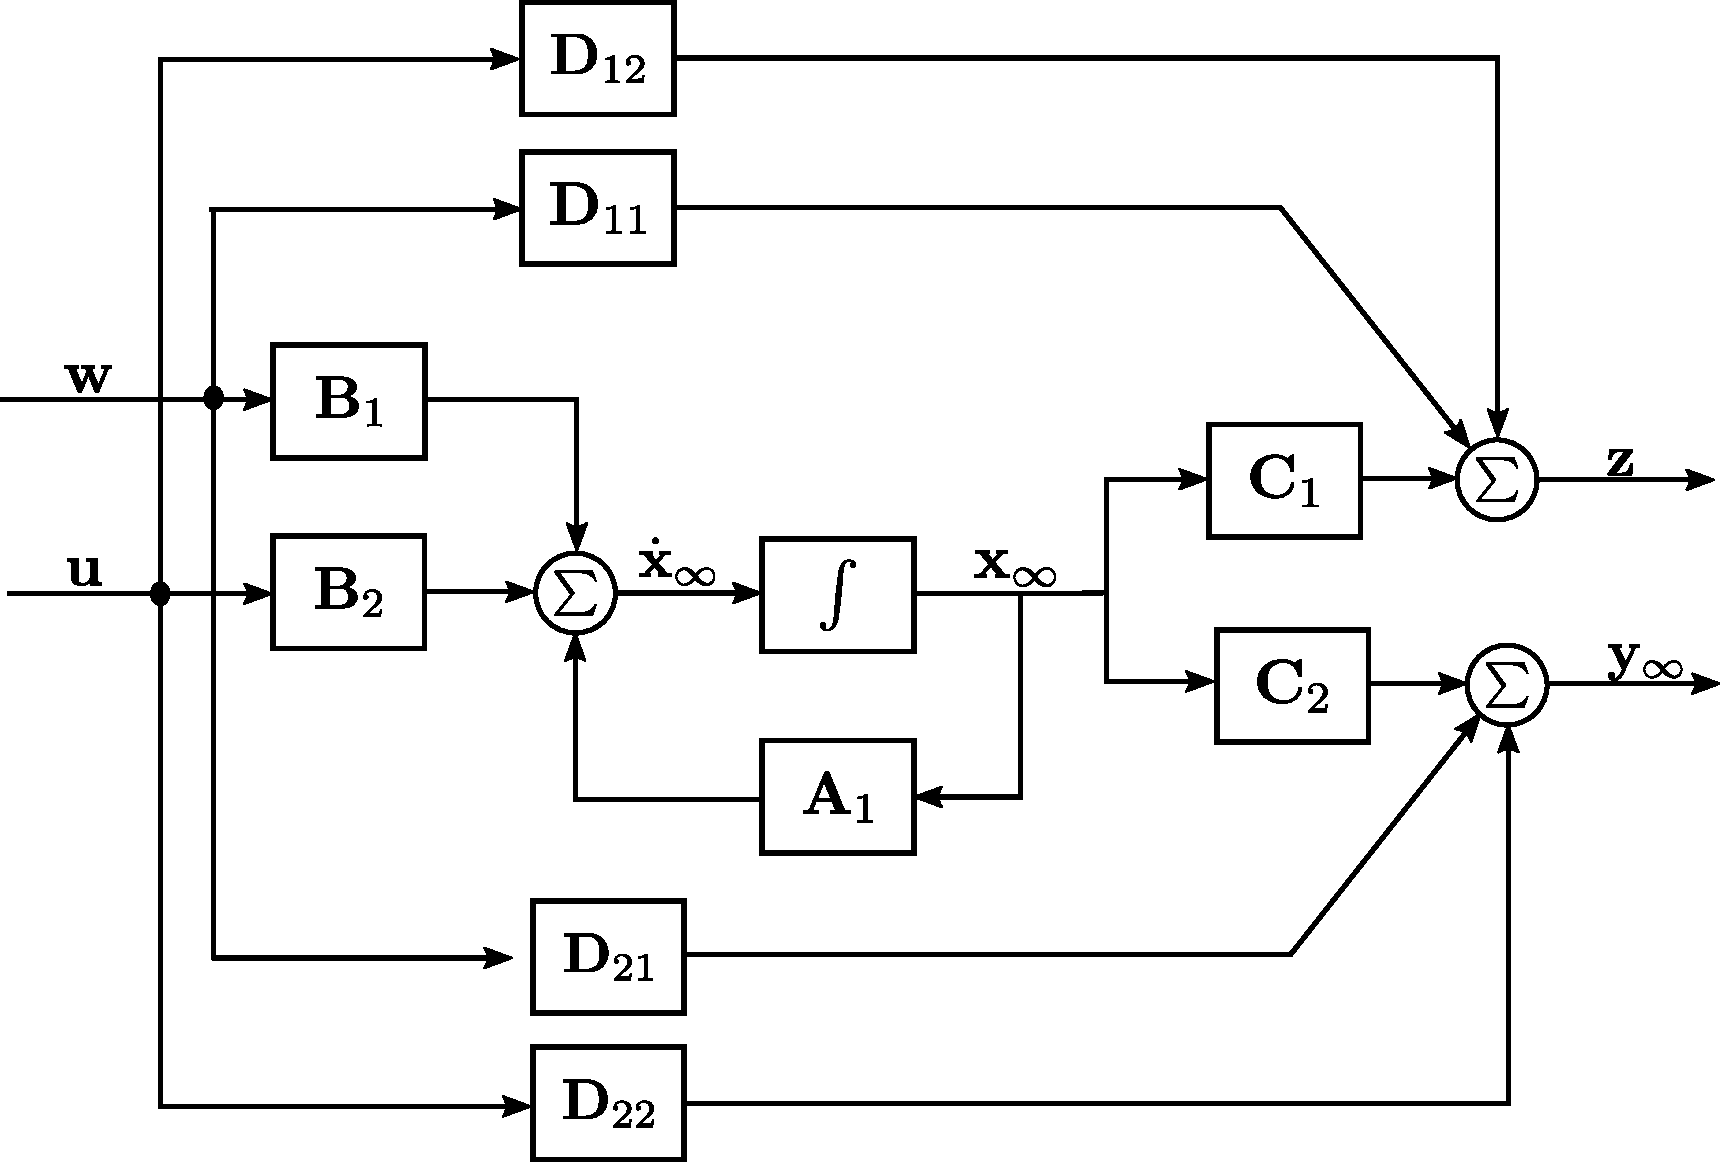
\includegraphics[width=0.55\linewidth]{figures/HinfDiag}
    \end{figure}
    \begin{minipage}[c][2.5cm]{\textwidth}
    \only<1|handout:1>{
    \begin{flalign}
    	\dot{\vec{x}}_\infty(t) &= \vec{A}_1 \vec{x}_\infty(t) + \vec{B}_1 \vec{w}(t) + \vec{B}_2 \vec{u}(t)\nonumber\\
    	\vec{z}(t) &= \vec{C}_1 \vec{x}_\infty(t) + \vec{D}_{11} \vec{w}(t) + \vec{D}_{12} \vec{u}(t)\nonumber\\
    	\vec{y}_\infty(t) &= \vec{C}_2 \vec{x}_\infty(t) + \vec{D}_{21} \vec{w}(t) + \vec{D}_{22} \vec{u}(t)\nonumber
    \end{flalign}}
    \only<2|handout:0>{
    \begin{flalign}	
    	\vec{u}(t) &= 
    	\begin{bmatrix}
    	F_1 & F_2 
    	\end{bmatrix}^\mathrm{T}\nonumber 
    \end{flalign}}
    \only<3|handout:0>{
    \begin{flalign}	
    	\vec{w}(t) &= 
    	\begin{bmatrix}
    	\psi_\mathrm{ref} & \dot{x}_\mathrm{b,ref} & F_\mathrm{wc} & \tau_\mathrm{wc} & F_\mathrm{wave} & \tau_\mathrm{wave}& n_{\psi} & n_{\dot{x}_\mathrm{b}}
    	\end{bmatrix}^\mathrm{T} \nonumber 
    \end{flalign}}
    \only<4|handout:0>{
    \begin{flalign}
    	\vec{y}_\infty(t) &= 
    	\begin{bmatrix}
    	\psi & \dot{x}_\mathrm{b} & \vec{x}_\mathrm{I}^\mathrm{T}
    	\end{bmatrix}^\mathrm{T}\nonumber 
    \end{flalign}}
    \only<5|handout:0>{
        \vspace{-0.55cm}
        \begin{flalign}
        \vec{x}_\infty(t) &=
        \begin{bmatrix}
        \psi & \dot{\psi} & \dot{x}_\mathrm{b} & x_{I_{\psi}} & x_{I_{\dot{x}_\mathrm{b}}} & x_{F_\mathrm{wc}} & x_{\tau_\mathrm{wc}} & x_{F_\mathrm{wave}} & x_{\tau_\mathrm{wave}} & x_{n_{\psi}}\ \ \  x_{n_{\dot{x}_\mathrm{b}}}
        \end{bmatrix}^\mathrm{T} \nonumber 
        \end{flalign}}
    \end{minipage}
\end{frame}

\begin{frame}{Inner Controller}{$\mathcal{H}_\infty$ Controller Design}
    \begin{itemize}
        \item Disturbance model
    \end{itemize}  
    \begin{figure}[H]
        \centering
        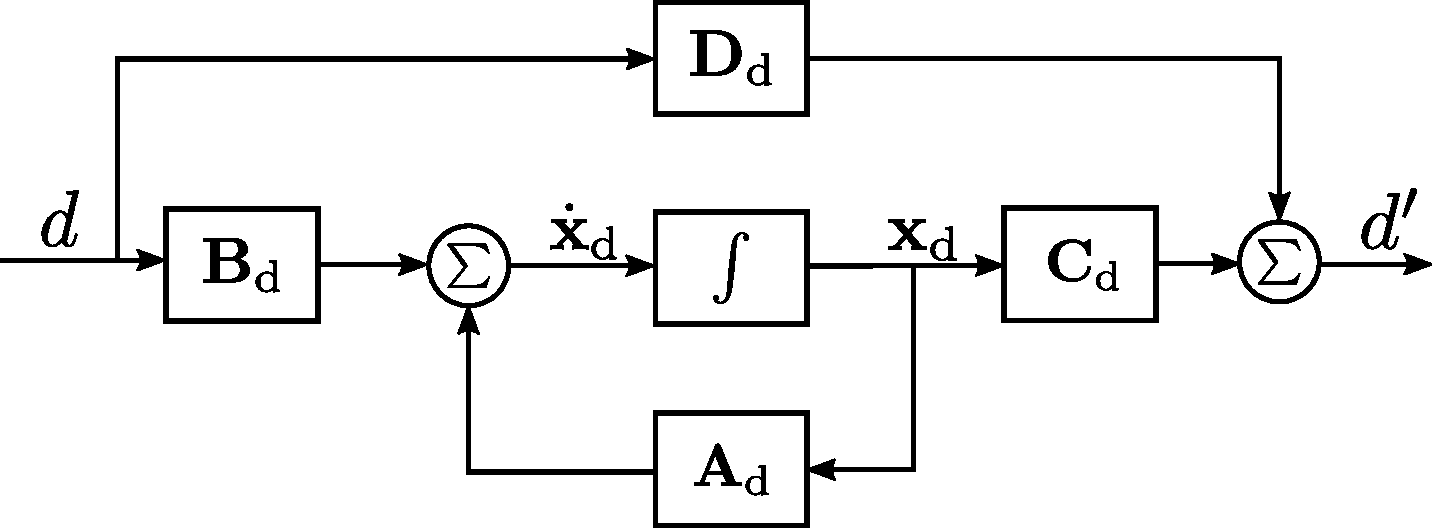
\includegraphics[width=0.6\linewidth]{figures/WeightDiag}
      \end{figure} 
      \begin{flalign}
      \frac{d'}{d}=\frac{a}{s+a} \rightarrow \dot{d}' = -a d' + a d \rightarrow \begin{cases} \dot{x}_\mathrm{d} = -a x_\mathrm{d} + a d \\ d' = x_\mathrm{d} \end{cases} \nonumber
      \end{flalign}    
\end{frame}
 
    
\begin{frame}<handout:0>{Inner Controller}{$\mathcal{H}_\infty$ Controller Design}
    \begin{itemize}
        \item System structure
    \end{itemize}
    \begin{figure}[H]
        \centering
        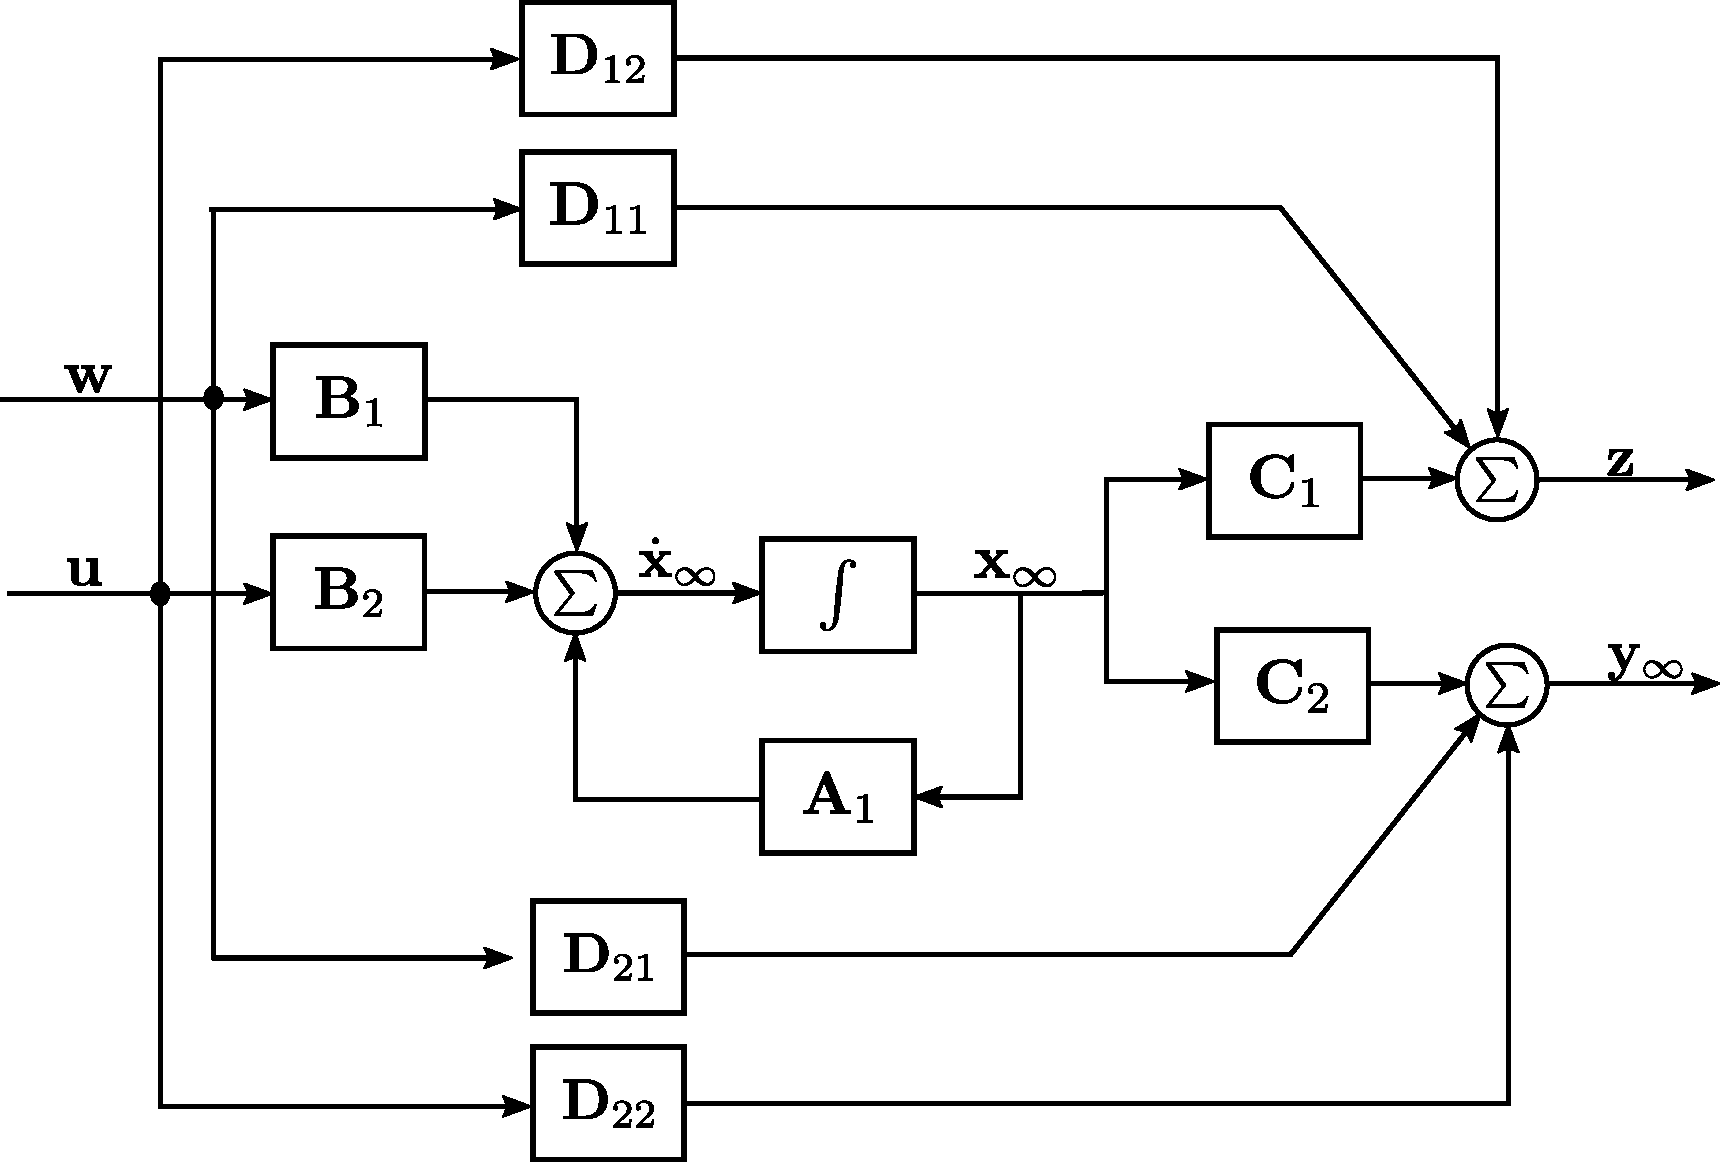
\includegraphics[width=0.55\linewidth]{figures/HinfDiag}
    \end{figure}
    \begin{minipage}[t][2.5cm]{\textwidth}
        \begin{flalign}	
        \vec{z}(t) &= 
        \begin{bmatrix}
        \vec{x}_\infty^\mathrm{T} & \vec{u}^\mathrm{T}
        \end{bmatrix}^\mathrm{T}\nonumber		
        \end{flalign}
    \end{minipage}
\end{frame}

\begin{frame}{Inner Controller}{$\mathcal{H}_\infty$ Controller Design}
    \begin{itemize}
        \item Controller design parameters ($\gamma$, $\vec{C}_1$, $\vec{D}_{12}$)
    \end{itemize}  
    \begin{minipage}{0.65\linewidth}
        \begin{flalign}
        \vec{C}_1 &=
        \begin{bmatrix}
            \vec{W}_\mathrm{x} & \vec{0}_{3\mathrm{x}2} &  \vec{0}_{3\mathrm{x}2} &  \vec{0}_{3\mathrm{x}2}  & \vec{0}_{3\mathrm{x}2} \\
            \vec{0}_{2\mathrm{x}3}  &  \vec{W}_\mathrm{I}  & \vec{0}_{2\mathrm{x}2} &  \vec{0}_{2\mathrm{x}2}  & \vec{0}_{2\mathrm{x}2} \\
            \vec{0}_{2\mathrm{x}3}  & \vec{0}_{2\mathrm{x}2} &  \vec{W}_\mathrm{wc} &  \vec{0}_{2\mathrm{x}2} &  \vec{0}_{2\mathrm{x}2} \\
            \vec{0}_{2\mathrm{x}3} &  \vec{0}_{2\mathrm{x}2}  & \vec{0}_{2\mathrm{x}2}  & \vec{W}_\mathrm{wave}  & \vec{0}_{2\mathrm{x}2} \\
            \vec{0}_{2\mathrm{x}3} &  \vec{0}_{2\mathrm{x}2}  & \vec{0}_{2\mathrm{x}2} &  \vec{0}_{2\mathrm{x}2} &  \vec{W}_\mathrm{noise} \\
            \vec{0}_{2\mathrm{x}3}  & \vec{0}_{2\mathrm{x}2}  & \vec{0}_{2\mathrm{x}2}  & \vec{0}_{2\mathrm{x}2} &  \vec{0}_{2\mathrm{x}2} \\
            \vec{0}_{2\mathrm{x}3}  & \vec{0}_{2\mathrm{x}2}  & \vec{0}_{2\mathrm{x}2}  & \vec{0}_{2\mathrm{x}2}  & \vec{0}_{2\mathrm{x}2} 
        \end{bmatrix}\nonumber
        \end{flalign} 
    \end{minipage}\hfill  
    \begin{minipage}{0.3\linewidth}
        \begin{flalign}
            \vec{D}_{12} &=
            \begin{bmatrix}
                \vec{0}_{2\mathrm{x}3} \\
                \vec{0}_{2\mathrm{x}2} \\
                \vec{0}_{2\mathrm{x}2} \\
                \vec{0}_{2\mathrm{x}2} \\
                \vec{0}_{2\mathrm{x}2} \\
                \vec{W}_\mathrm{u}
            \end{bmatrix} \nonumber
        \end{flalign}
    \end{minipage}\hfill 
 
\end{frame}


\begin{frame}{Inner Controller}{$\mathcal{H}_\infty$ Controller Design}
    \begin{itemize}
        \item Feedback gain
    \end{itemize}
    \begin{flalign}
        \vec{X}_\infty = Ric
        \begin{bmatrix}
        \vec{A}_1 & \gamma^{-2}\vec{B}_1\vec{B}_1^\mathrm{T} - \vec{B}_2\vec{B}_2^\mathrm{T} \\
        -\vec{C}_1^\mathrm{T}\vec{C}_1 & -\vec{A}_1^\mathrm{T}
        \end{bmatrix} \nonumber
    \end{flalign}
    \begin{flalign}
        \vec{F}_\infty = -\vec{B}_2^\mathrm{T}\vec{X}_\infty \nonumber
    \end{flalign}
\end{frame}


\begin{frame}<handout:0>{Agenda}{}
  \begin{itemize}
    \item Introduction
%    \begin{itemize}
%      \item[-] The System
%      \item[-] Task
%    \end{itemize}
    \item Modeling
    \begin{itemize}
%      \item[-] Conventions and Assumptions
      \item[-] Newton's Method
      \item[-] Energy Method
%      \item[-] Friction Model
    \end{itemize}
    \item Nonlinear Control
    \begin{itemize}
%      \item[-] System Transformation
      \item[-] Sliding Mode
%      \item[-] Simulation
    \end{itemize}
    \item Trajectory Planning
%    \begin{itemize}
%      \item[-] System
%      \item[-] Integral of System
%      \item[-] Trajectories
%    \end{itemize}
    \item Results
%    \begin{itemize}
%      \item[-] Sliding Mode
%      \item[-] Trajectory Planning
%    \end{itemize}
  \end{itemize}
\end{frame}


%-------Introduction-----------------------------------------------------------


\begin{frame}{Introduction}{The System}
  \begin{figure}[H]
    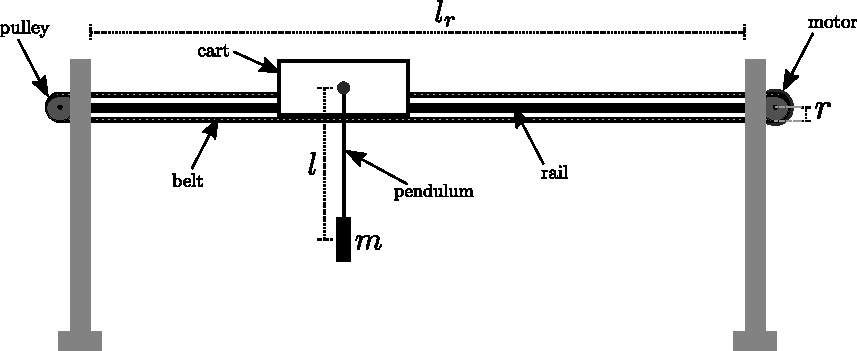
\includegraphics[width=1\textwidth]{figures/systemSetup}
  \end{figure}
\end{frame}

\begin{frame}{Introduction}{Task}
  \begin{figure}[H]
    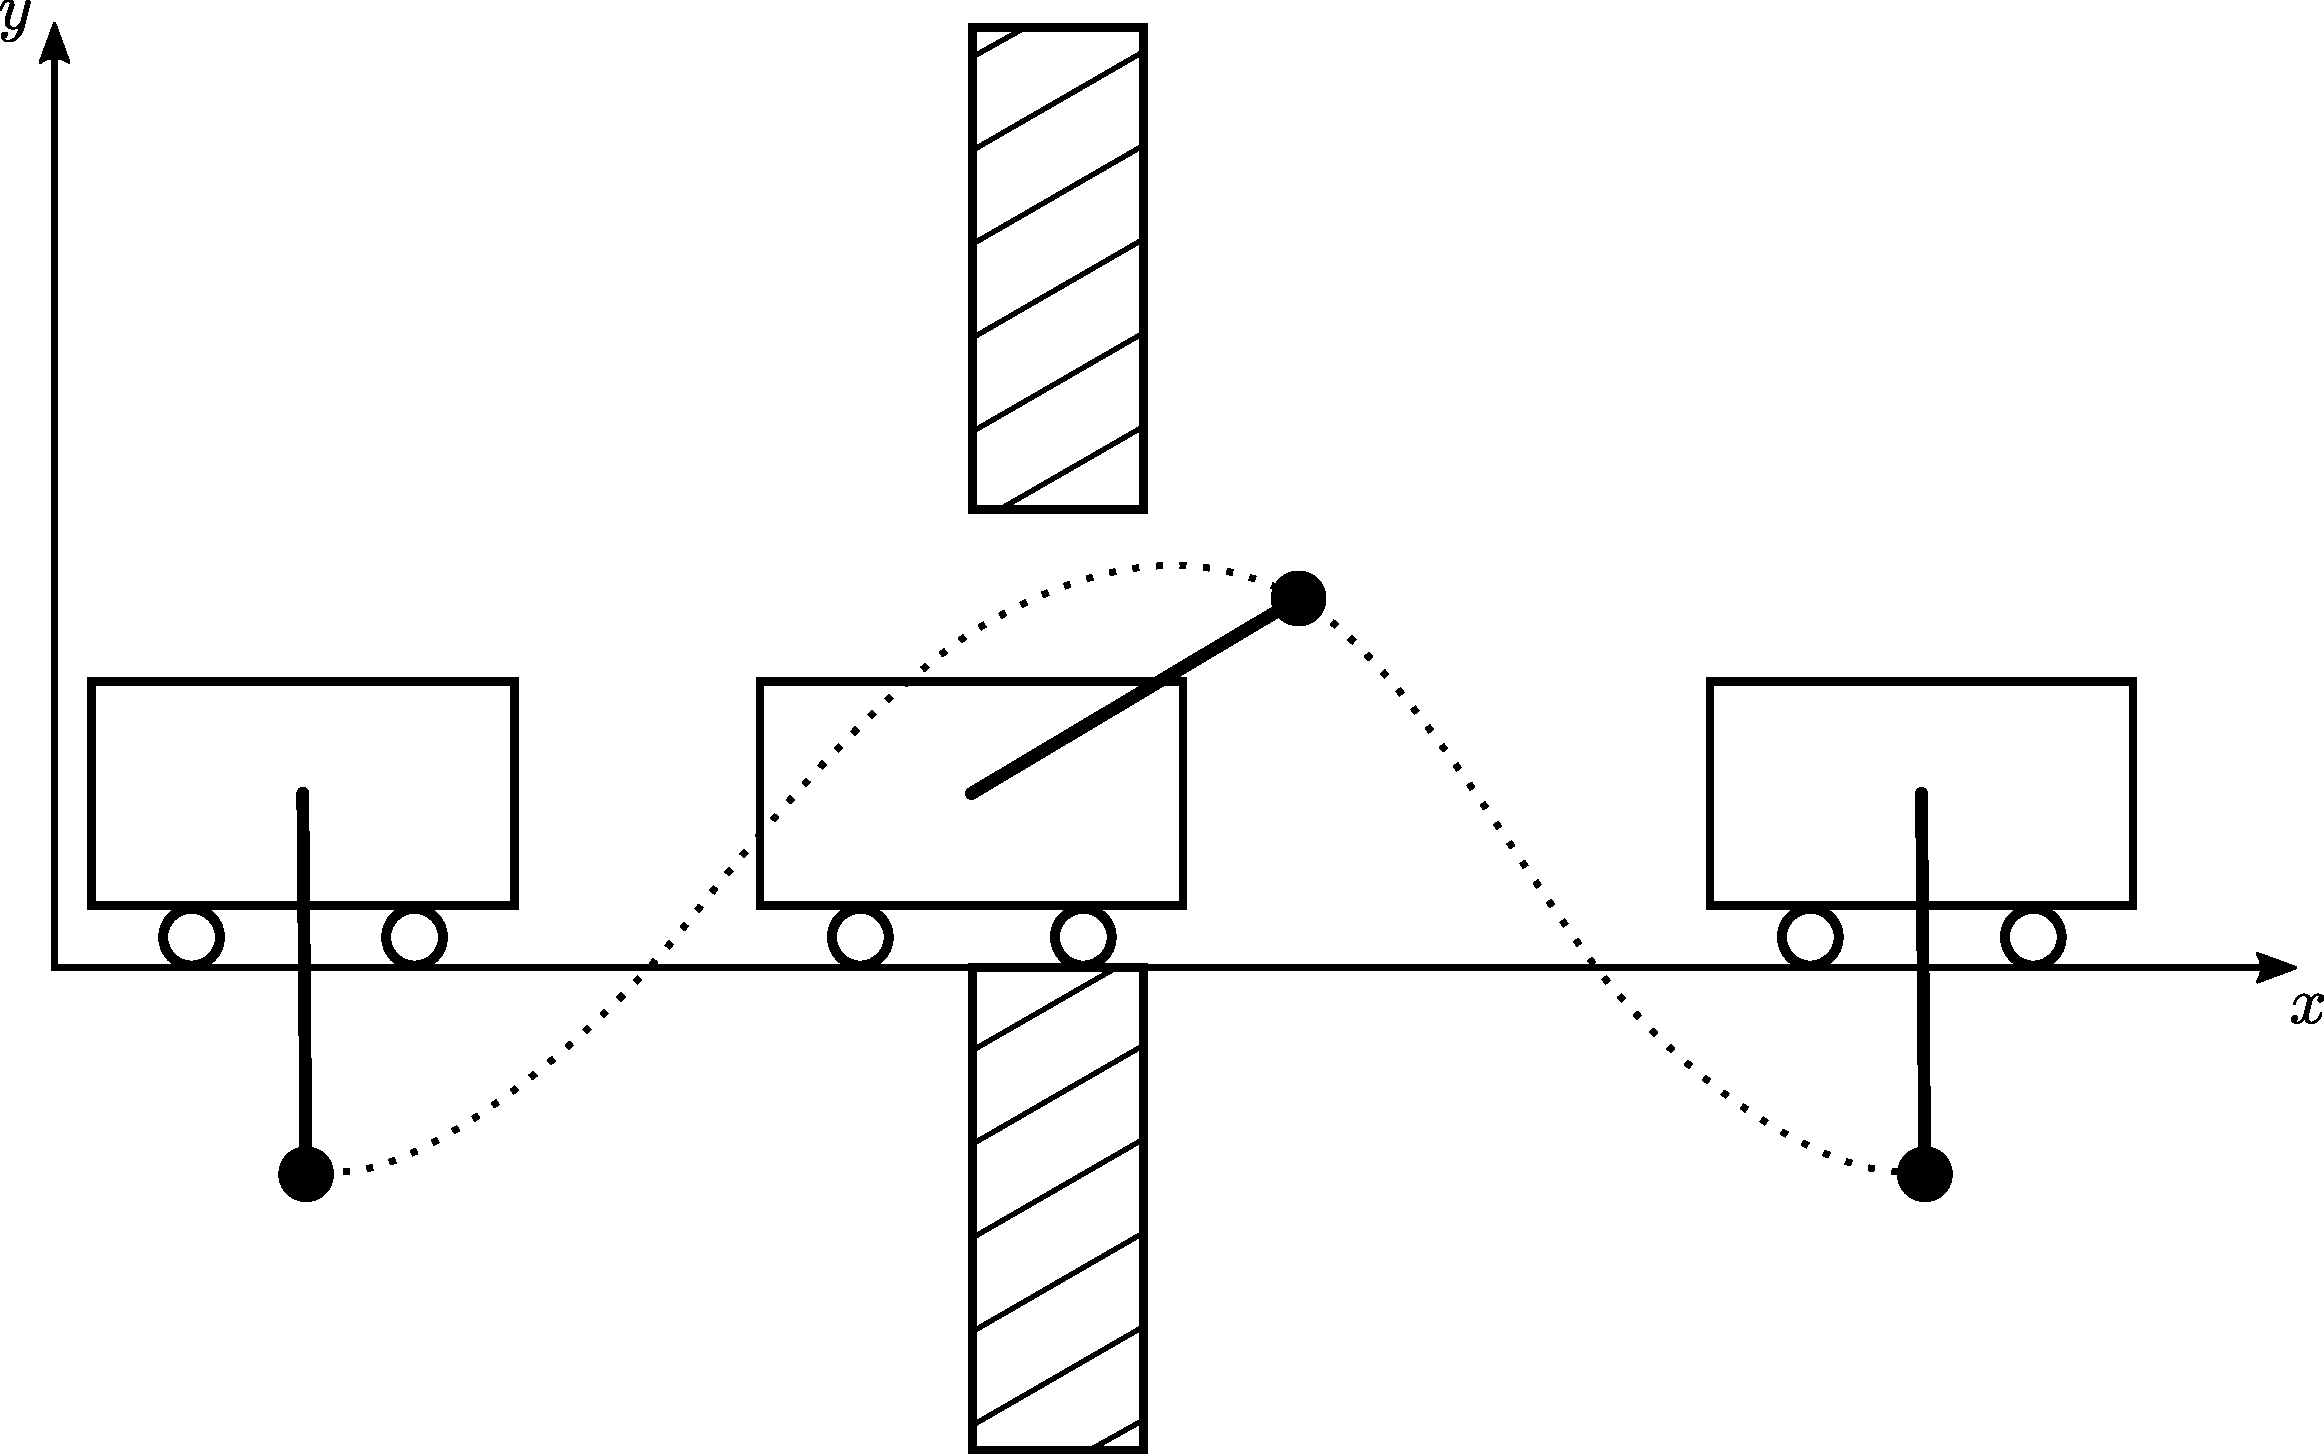
\includegraphics[width=.85\textwidth]{figures/systemTask}
  \end{figure}
\end{frame}


%-------Modelling-----------------------------------------------------------


\begin{frame}{Modeling}{Conventions and Assumptions}
  \small
  \vspace{-1cm}
  \begin{figure}[H]
    \begin{minipage}{0.45\linewidth}
      \begin{figure}[H]
        \hspace{-3cm}
        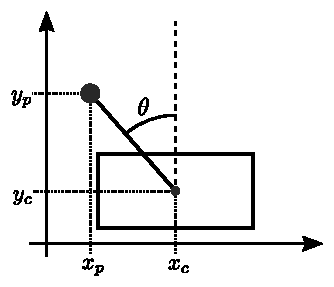
\includegraphics[width=1\linewidth]{figures/excessiveCoordinates}
      \end{figure}        
    \end{minipage}\hspace{-1cm}
    \begin{minipage}{0.45\linewidth}
      \begin{figure}[H]
        \vspace{.2cm}
        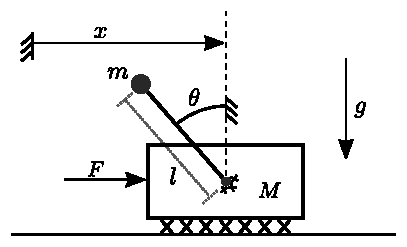
\includegraphics[width=1.3\linewidth]{figures/mechanicalDrawing}
      \end{figure}\hspace{1cm}
    \end{minipage}
  \end{figure}
  \vspace{-.3cm}
  \begin{flalign}
    \hspace{-10pt}
    \begin{cases}
      x_c &=  x  \\
      y_c &=  0  
    \end{cases} & \nonumber
    \hspace{5pt}
    \begin{cases}
      x_p &=  x - l\sin \theta \\
      y_p &=  l\cos \theta
    \end{cases} & \nonumber
    \hspace{-4pt}
    \begin{cases}
      \dot{x}_p &= \dot{x} - l\cos \theta \dot{\theta} \\
      \dot{y}_p &= -l\sin \theta \dot{\theta}
    \end{cases} &\nonumber
    \hspace{5pt}
    \begin{cases}
      \ddot{x}_p = \ddot{x} + l \sin \theta \dot{\theta}^2 - l\cos \theta \ddot{\theta} \\
      \ddot{y}_p = -l\cos \theta \dot{\theta}^2  -l\sin \theta \ddot{\theta}
    \end{cases}  & \nonumber
  \end{flalign}
  \normalsize
\end{frame}

\begin{frame}{Modeling}{Newton's Method}
  \small
  \begin{figure}[H]
    \vspace{-1cm}\hspace{.1cm}
    \begin{minipage}{0.45\linewidth}
      \begin{figure}[H]
        \hspace{-2cm}
        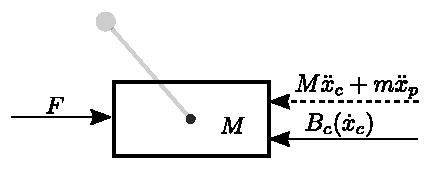
\includegraphics[width=1.2\linewidth]{figures/freeBodyCart}
      \end{figure}        
    \end{minipage}\hspace{-1cm}
    \begin{minipage}{0.45\linewidth}
      \begin{figure}[H]
        \vspace{-.25cm}
        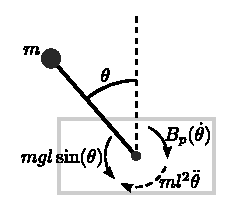
\includegraphics[width=.8\linewidth]{figures/freeBodyPendulum}
      \end{figure}\hspace{1cm}
    \end{minipage}
  \end{figure}
  %
  \begin{minipage}{0.45\linewidth}
    \vspace{-1.3cm}
    \begin{flalign} \hspace{.1cm}
      M\ddot{x}_c + m\ddot{x}_p &= F - B_c(\dot{x}_c) & \nonumber
    \end{flalign}
  \end{minipage}
  \begin{minipage}{0.45\linewidth}
    \vspace{-1.5cm}
    \begin{flalign} \hspace{7cm}
      ml^2 \ddot{\theta} &= mgl \sin \theta - B_p(\dot{\theta}) & \nonumber \\
      - ml\ddot{x}_p \cos \theta - ml\ddot{y}_p \sin \theta &=  mgl \sin \theta - B_p(\dot{\theta}) & \nonumber
    \end{flalign}
  \end{minipage}

  \begin{flalign}
    \begin{cases}
      ml^2 \ddot{\theta} - ml\cos \theta \ddot{x} - mgl \sin \theta &= - B_p(\dot{\theta}) \\
      ( M + m ) \ddot{x} + ml\sin \theta \dot{\theta}^2 - ml\cos \theta \ddot{\theta} &= F - B_c(\dot{x}) 
    \end{cases} & \nonumber
  \end{flalign}
  \normalsize
\end{frame}


\begin{frame}{Modeling}{Energy Method}
  \small
  \begin{minipage}{0.45\linewidth}
    \vspace{-.3cm}
    \begin{flalign} \hspace{.1cm}
      U &= mg\overbrace{l( 1 + \cos \theta )}^{h} + 0  \nonumber  &  \\
      T &= \tfrac{1}{2} m \dot{x}_p^2 + \tfrac{1}{2} m \dot{y}_p^2  + \tfrac{1}{2} M \dot{x}_c^2 \nonumber & 
    \end{flalign}
  \end{minipage}
  \begin{minipage}{0.45\linewidth}
    \vspace{-1.5cm}
    \begin{flalign}\hspace{5cm}
      U &= mgl( 1 + \cos \theta )   & \nonumber  \\
      T &= \frac{1}{2} ( M + m ) \dot{x}^2 - m \dot{x} l \cos \theta \dot{\theta} + \frac{1}{2} m l^2 \dot{\theta}^2 & \nonumber
    \end{flalign}
  \end{minipage}
  \begin{flalign}
    \cal{L} &= T - U & \nonumber \\ 
    \cal{L} &= \tfrac{1}{2} ( M + m ) \dot{x}^2 - m \dot{x} l \cos \theta \dot{\theta} + \tfrac{1}{2} m l^2 \dot{\theta}^2 - m g l( 1 + \cos \theta ) &  \nonumber
  \end{flalign}
  \begin{flalign}
    \frac{d}{dt}  \frac{\partial \cal{L}}{\partial \dot{\vec{q}}} - \frac{\partial \cal{L}}{\partial \vec{q}}  &=  \vec{Q}  && \nonumber
  \end{flalign}
  \begin{flalign}
    \begin{cases}
      ml^2 \ddot{\theta} - ml\cos \theta \ddot{x} - mgl \sin \theta &= - B_p(\dot{\theta}) \\
      ( M + m ) \ddot{x} + ml\sin \theta \dot{\theta}^2 - ml\cos \theta \ddot{\theta} &= F - B_c(\dot{x}) 
    \end{cases} && \nonumber
  \end{flalign}
  \normalsize
\end{frame}

\begin{frame}{Modeling}{Friction Model}
  \small
  \vspace{-1cm}
  \begin{figure}[H]\hspace{-3cm}
    \begin{minipage}{0.3\linewidth}
      \begin{figure}[H]
        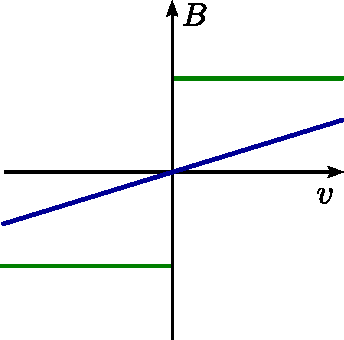
\includegraphics[width=.8\linewidth]{figures/coulombViscous1}
      \end{figure}        
    \end{minipage}%\hspace{-1cm}
    \begin{minipage}{0.3\linewidth}
      \begin{figure}[H]
        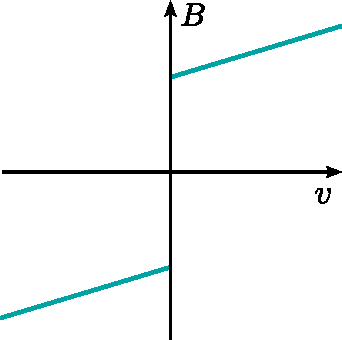
\includegraphics[width=.8\linewidth]{figures/coulombViscous2}
      \end{figure}
    \end{minipage}%\hspace{-1cm}
    \begin{minipage}{0.3\linewidth}
      \begin{figure}[H]
        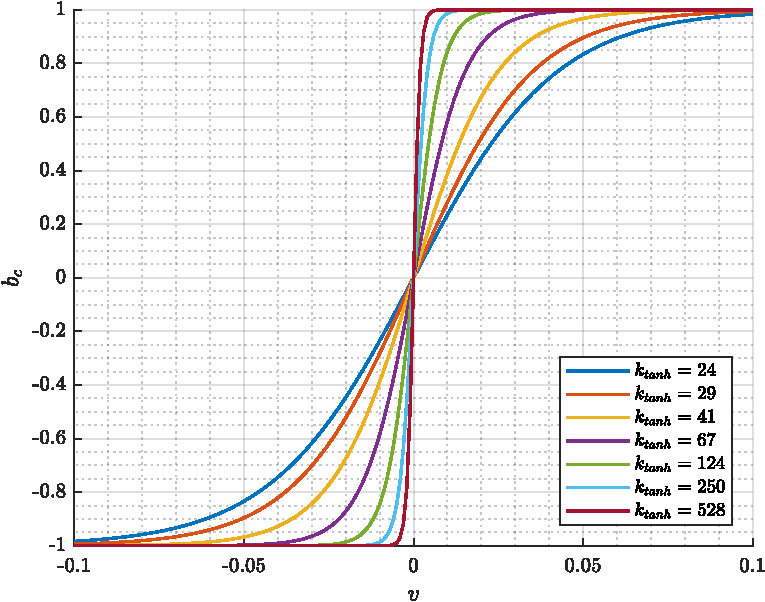
\includegraphics[width=1.7\linewidth]{figures/tanhApprox}
      \end{figure}
    \end{minipage}
  \end{figure}
  \vspace{-.2cm}
  \begin{minipage}{0.3\linewidth}
    \begin{flalign}
      B_p(\dot{\theta}) &= b_{p,v} \dot{\theta} + \text{sgn}(\dot{\theta}) b_{p,c} & \nonumber \\
      B_c(\dot{x})      &= b_{c,v} \dot{x}      + \text{sgn}(\dot{x}) b_{c,c} & \nonumber
    \end{flalign}
  \end{minipage}\hspace{1.7cm}
  \begin{minipage}{0.3\linewidth}
    \begin{flalign}
      B_p(\dot{\theta}) &= b_{p,v} \dot{\theta} + \tanh(\text{k}_\text{tanh}\dot{\theta}) b_{p,c}  & \nonumber \\
      B_c(\dot{x})      &= b_{c,v} \dot{x}      + \tanh(\text{k}_\text{tanh}\dot{x}) b_{c,c}   &  \nonumber
    \end{flalign}
  \end{minipage}
  \normalsize
\end{frame}


%-------Nonlinear Control--(System Transformation)-----------------------------


\begin{frame}{Nonlinear Control}{System Transformation}
\small
\vspace{-.5cm}
%\begin{flalign}
%\dot{\vec{\eta}} &=  f_a(\vec{\eta},\vec{\xi}) \nonumber  \\
%\dot{\vec{\xi}}  &=  f_b(\vec{\eta},\vec{\xi}) + g_b(\vec{\eta},\vec{\xi}) F  & \nonumber
%\end{flalign}
\begin{flalign}
\begin{bmatrix}
m l^2              & -m l \cos \theta  \\
-m l \cos \theta   & M + m
\end{bmatrix}
\begin{bmatrix}
\ddot{\theta}  \\
\ddot{x}
\end{bmatrix}
+
\begin{bmatrix}
0  \\
m l \sin \theta \dot{\theta}^2
\end{bmatrix}
+
\begin{bmatrix}
B_p(\dot{\theta})  \\
B_c(\dot{x})
\end{bmatrix}
+
\begin{bmatrix}
-m g l \sin \theta  \\
0
\end{bmatrix}
&=
\begin{bmatrix}
0  \\
F
\end{bmatrix}  & \nonumber
\end{flalign}
%
\vspace{.5cm}
\begin{minipage}{1\linewidth}\hspace{7cm}
  $[\ x_1\ x_2\ x_3\ x_4\ ]^T = [\ \theta\ x\ \dot{\theta}\ \dot{x}\ ]^T $
\end{minipage}
%
\vspace{-1.2cm}
\begin{flalign}
&\vec{M}(\vec{q})\ddot{\vec{q}} + \vec{C}(\vec{q},\dot{\vec{q}}) + \vec{B}(\dot{\vec{q}}) + \vec{G}(\vec{q}) = \vec{F}  & \nonumber \\
&\ddot{\vec{q}}
=
\vec{M}^{-1}(\vec{q})
\left(
\vec{F} -\vec{C}(\vec{q},\dot{\vec{q}}) -\vec{B}(\dot{\vec{q}}) -\vec{G}(\vec{q})
\right)  \nonumber &
\end{flalign}
%
\begin{flalign}
\begin{bmatrix}
\dot{x_1} \\
\dot{x_2} \\
\dot{x_3} \\
\dot{x_4}
\end{bmatrix}
&=
\begin{bmatrix}
x_3  \\
x_4  \\
\vec{M}^{-1}(x_1)
\left(
-\vec{C}(x_1,x_3) -\vec{B}(x_3,x_4) -\vec{G}(x_1)
\right)
\end{bmatrix}
+
\begin{bmatrix}
0  \\
0  \\
\vec{M}^{-1}(x_1)   \begin{bmatrix}
0  \\
F
\end{bmatrix}
\end{bmatrix}  & \nonumber \\
%
%
\begin{bmatrix}
\dot{x_1} \\
\dot{x_2} \\
\dot{x_3} \\
\dot{x_4}
\end{bmatrix}
&=
\underbrace{ 
  \begin{bmatrix}
  x_3  \\
  x_4  \\
  f_1(\vec{x})  \\
  f_2(\vec{x})
  \end{bmatrix}
}_{f(\vec{x})}
+
\underbrace{ 
  \begin{bmatrix}
  0  \\
  0  \\
  \frac{\cos x_1}{l (M + m - m \cos^2 x_1)} \\
  \frac{1}{M + m - m \cos^2 x_1}
  \end{bmatrix}
}_{g(\vec{x})}
F  & \nonumber
\end{flalign}
\normalsize
\end{frame}

\begin{frame}{Nonlinear Control}{System Transformation}
  \small
    \vspace{-.4cm}
     $y = h(\vec{x}) = x_1$
     \vspace{-.1cm}
    \begin{flalign}
      \dot{y}  &= \dot{x_1} = x_3 & \nonumber \\
      \ddot{y} &= \dot{x_3} = f_1(\vec{x}) + \frac{\cos x_1}{l (M + m - m \cos^2 x_1)} F \ \ \ \ \Rightarrow \ \ \ \ \rho = 2 & \nonumber
    \end{flalign}
    \vspace{-.5cm}
    \begin{flalign}
      T(\vec{x})
      &=
      \begin{bmatrix}
      \vec{\phi}(\vec{x}) \\  %these are dotted lines, yea, that's LaTeX for ya, go figure..
      \begin{picture} (0,0)(0,0) \multiput(1,8)(4,0){5}{\line(2,0){2}} \end{picture}
      \vec{\psi}(\vec{x})
      \end{bmatrix} 
      =
      \begin{bmatrix}
      \phi_1(\vec{x}) \\
      \phi_2(\vec{x}) \\  %these are dotted lines, yea, that's LaTeX for ya, go figure..
      \begin{picture} (0,0)(0,0) \multiput(-3.4,8)(4.5,0){6}{\line(2,0){2}} \end{picture}
      h(\vec{x}) \\
      L_f h(\vec{x})
      \end{bmatrix}
      =
      \begin{bmatrix}
      \phi_1(\vec{x}) \\
      \phi_2(\vec{x}) \\  %these are dotted lines, yea, that's LaTeX for ya, go figure..
      \begin{picture} (0,0)(0,0) \multiput(-7,8)(4,0){6}{\line(2,0){2}} \end{picture}
      x_1 \\
      x_3
      \end{bmatrix} & \nonumber
    \end{flalign}
    \vspace{-.5cm}
    \begin{flalign}
      \frac{\partial \phi_i}{\partial \vec{x} }  g(\vec{x})  &= 0 \ , \ \ \text{for} \ 1 \leq i \leq 2 & \nonumber
    \end{flalign}
    \vspace{-.5cm}
    \begin{flalign}
      \frac{\partial \phi_2}{\partial x_3 } \cdot \frac{\cos x_1}{l (M + m - m \cos^2 x_1)}  &+  \frac{\partial \phi_2}{\partial x_4 } \cdot \frac{l}{l(M + m - m \cos^2 x_1)}  =  0  \nonumber & 
    \end{flalign}
    \begin{minipage}{.25\linewidth}
      \vspace{-.35cm}
      \begin{flalign}
        \frac{\partial \phi_2}{\partial x_3 } &=  l & \nonumber \\
        \frac{\partial \phi_2}{\partial x_4 } &=  -\cos x_1  \nonumber &
      \end{flalign}
    \end{minipage}
    \begin{minipage}{.60\linewidth}
      \vspace{-.35cm}
      \begin{flalign}
        \phi_2 &=  l \int  d x_3  - \cos x_1 \int  d x_4  & \nonumber \\
        \phi_2 &=  l x_3 - \cos x_1 x_4 + \mathrm{C}_1 \ \ ,\ \ \ \phi(0)=0\ \ \ \Rightarrow\ \ \  \mathrm{C}_1=0 \nonumber &
      \end{flalign}
    \end{minipage}
  \normalsize
\end{frame}

\begin{frame}{Nonlinear Control}{System Transformation}
\small
\begin{minipage}{.37\linewidth}
  \begin{flalign}
    T(\vec{x})
    &=
    \begin{bmatrix}
      x_2 \\
      %\frac{l}{\cos x_1} x_3  - x_4 \\ 
      l x_3 - \cos x_1 x_4 \\
      x_1 \\
      x_3
    \end{bmatrix} \ \ \ ,  & \nonumber
  \end{flalign}
\end{minipage}
\begin{minipage}{.45\linewidth}
  \begin{flalign}
    \frac{d }{d t } T(\vec{x})
    &=
    \begin{bmatrix}
      \dot{x}_2 \\
      %\frac{l \sin x1}{\cos^2 x_1} \dot{x}_1 x_3 +  \frac{l}{\cos x_1} \dot{x}_3 - \dot{x}_4 \\ 
      l \dot{x}_3 + \sin x_1 x_4 \dot{x}_1 - \cos x_1 \dot{x}_4 \\
      \dot{x}_1 \\
      \dot{x}_3
    \end{bmatrix}  & \nonumber
  \end{flalign}
\end{minipage}
\vspace{.3cm}
\begin{flalign}
\begin{bmatrix}
\dot{\eta}_1   \\
\dot{\eta}_2   \\
\dot{\eta}_3   \\  %these are dotted lines, yea, that's LaTeX for ya, go figure..
\begin{picture} (0,0)(0,0) \multiput(-2,9.5)(4,0){3}{\line(2,0){2}} \end{picture}
\dot{\xi}
\end{bmatrix}
&=
\overbrace{
  \underbrace{
    \begin{bmatrix}
    x_4    \\
    %\frac{l \sin x1}{\cos^2 x_1} x_3^2 +  \tfrac{l}{\cos x_1} f_1(\vec{x})  - f_2(\vec{x}) \\ 
    \sin x_1 x_4 x_3 + l f_1(\vec{x}) - \cos x_1 f_2(\vec{x})  \\
    x_3    \\ %these are dotted lines, yea, that's LaTeX for ya, go figure..
    \begin{picture} (0,0)(0,0) \multiput(-50,9)(4,0){30}{\line(2,0){2}} \end{picture}
    f_1(\vec{x}) 
    \end{bmatrix}
  }_{f_b} }^{f_a}
+
\underbrace{
  \begin{bmatrix}
  0    \\
  0    \\
  0    \\  %these are dotted lines, yea, that's LaTeX for ya, go figure..
  \begin{picture} (0,0)(0,0) \multiput(4,9.5)(4,0){13}{\line(2,0){2}} \end{picture}
  \frac{\cos x_1}{l (M + m - m \cos^2 x_1)}
  \end{bmatrix}
}_{g_b} F  & \nonumber
\end{flalign}
\begin{flalign}
  \dot{\vec{\eta}} &=  f_a(\vec{\eta},\xi)  \nonumber  \\
  \dot{\xi}        &=  f_b(\vec{\eta},\xi) + g_b(\vec{\eta},\xi) F  \nonumber &
\end{flalign}
\normalsize
\end{frame}


\begin{frame}{Nonlinear Control}{System Transformation}
\small
\vspace{-.4cm}
\begin{flalign}
  \begin{bmatrix}
    \eta_1   \\
    \eta_2   \\
    \eta_3   \\
    \xi
  \end{bmatrix} 
  &=
  \begin{bmatrix}
    x_2 \\
    %\frac{l}{\cos x_1} x_3  - x_4 \\
    l x_3 - \cos x_1 x_4 \\
    x_1 \\
    x_3
  \end{bmatrix} \ \ \ \ \ \ \Rightarrow \ \ \ \ \ \ \ 
  \begin{bmatrix}
    x_1   \\
    x_2   \\
    x_3   \\
    x_4
  \end{bmatrix} 
  =
  \begin{bmatrix}
    \eta_3 \\
    \eta_1 \\ 
    \xi    \\
    %\frac{l}{\cos \eta_3} \xi -\eta_2
    \frac{l\xi - \eta_2}{\cos \eta_3}
  \end{bmatrix}  \nonumber &
\end{flalign}
\vspace{.5cm}
\begin{flalign}
  \begin{bmatrix}
    \dot{\eta}_1   \\
    \dot{\eta}_2   \\
    \dot{\eta}_3   \\
    \dot{\xi}
  \end{bmatrix} 
  &=
  \begin{bmatrix}
    %\frac{l}{\cos \eta_3} \xi -\eta_2    \\
    \frac{l\xi - \eta_2}{\cos \eta_3}     \\
    %\frac{l \sin \eta_3}{\cos^2 \eta_3} \xi^2 +  \tfrac{l}{\cos \eta_3} f_1(\vec{\eta},\xi)  - f_2(\vec{\eta},\xi) \\ 
    \frac{\sin \eta_3}{\cos \eta_3}(l\xi - \eta_2) \xi + l f_1(\vec{\eta},\xi) - \cos \eta_3 f_2(\vec{\eta},\xi)    \\
    \xi   \\
    f_1(\vec{\eta},\xi) 
  \end{bmatrix} 
  + 
  \begin{bmatrix}
    0    \\
    0    \\
    0    \\ 
    \frac{\cos \eta_3}{l (M + m - m \cos^2\eta_3)}
  \end{bmatrix} F  \nonumber &
\end{flalign}
\normalsize
\end{frame}

%-------Nonlinear Control--(Sliding Mode)-----------------------------

\begin{frame}{Nonlinear Control}{Sliding Mode}
  \vspace{-.4cm}
  \begin{flalign}
    s &=   \xi - \phi(\vec{\eta}) = 0   & \nonumber
  \end{flalign}
  \begin{flalign}
    \dot{\vec{\eta}} &=  f_a(\vec{\eta},\phi(\vec{\eta}))   & \nonumber
  \end{flalign}
  \begin{flalign}
    A &= \frac{\partial \dot{\vec{\eta}}}{\partial \vec{\eta}} \whereThree{\vec{\eta}=\vec{0}\ \ \ \ }{\xi=0\ \ \ \ }{\mathrm{k}_\mathrm{tanh}=1} \ 
    =
    \begin{bmatrix}
      0 & -1                  & 0 \\
      0 & \frac{g_{p,c}}{l m} & g \\
      0 & 0                   & 0 
    \end{bmatrix}   \ \ \ , \ \ \
      B = \frac{\partial \dot{\vec{\eta}}}{\partial \xi} \whereThree{\vec{\eta}=\vec{0}\ \ \ \ }{\xi=0\ \ \ \ }{\text{k}_\text{tanh}=1} \ 
    =
    \begin{bmatrix}
      l  \\
      \frac{-b_{p,v}-b_{p,c}}{l m}  \\
      1  
    \end{bmatrix}   \nonumber & 
  \end{flalign}
  \begin{flalign}
    \phi(\vec{\eta}) &=   - \vec{k} \vec{\eta}  \nonumber &
  \end{flalign}
\end{frame}

\begin{frame}{Nonlinear Control}{Sliding Mode}
\begin{minipage}{\textwidth}
  \begin{minipage}{0.50\textwidth}
    \begin{figure}[H]
      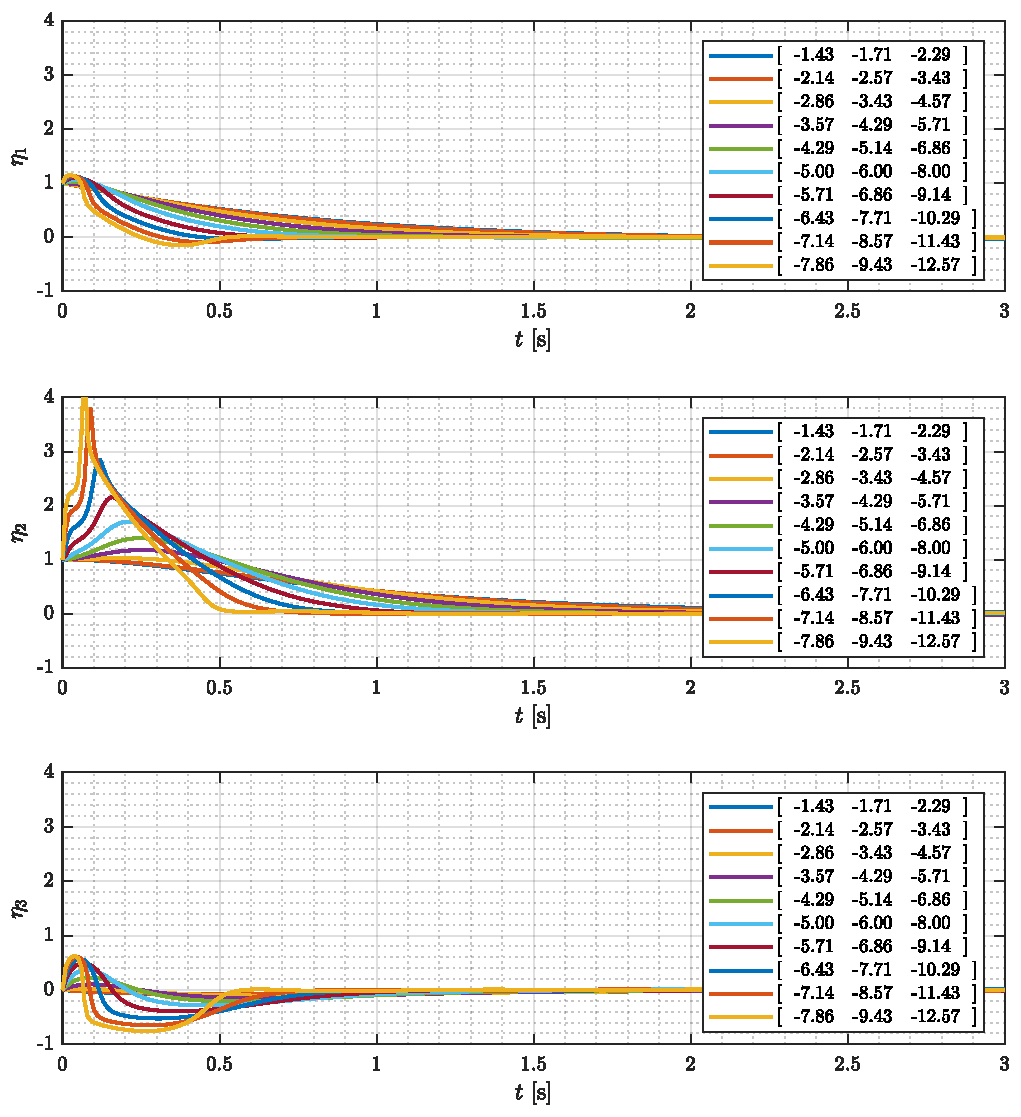
\includegraphics[width=\textwidth]{figures/reducedOrderControlMany}
    \end{figure}
  \end{minipage}
  \begin{minipage}{0.50\textwidth}
    \begin{figure}[H]
      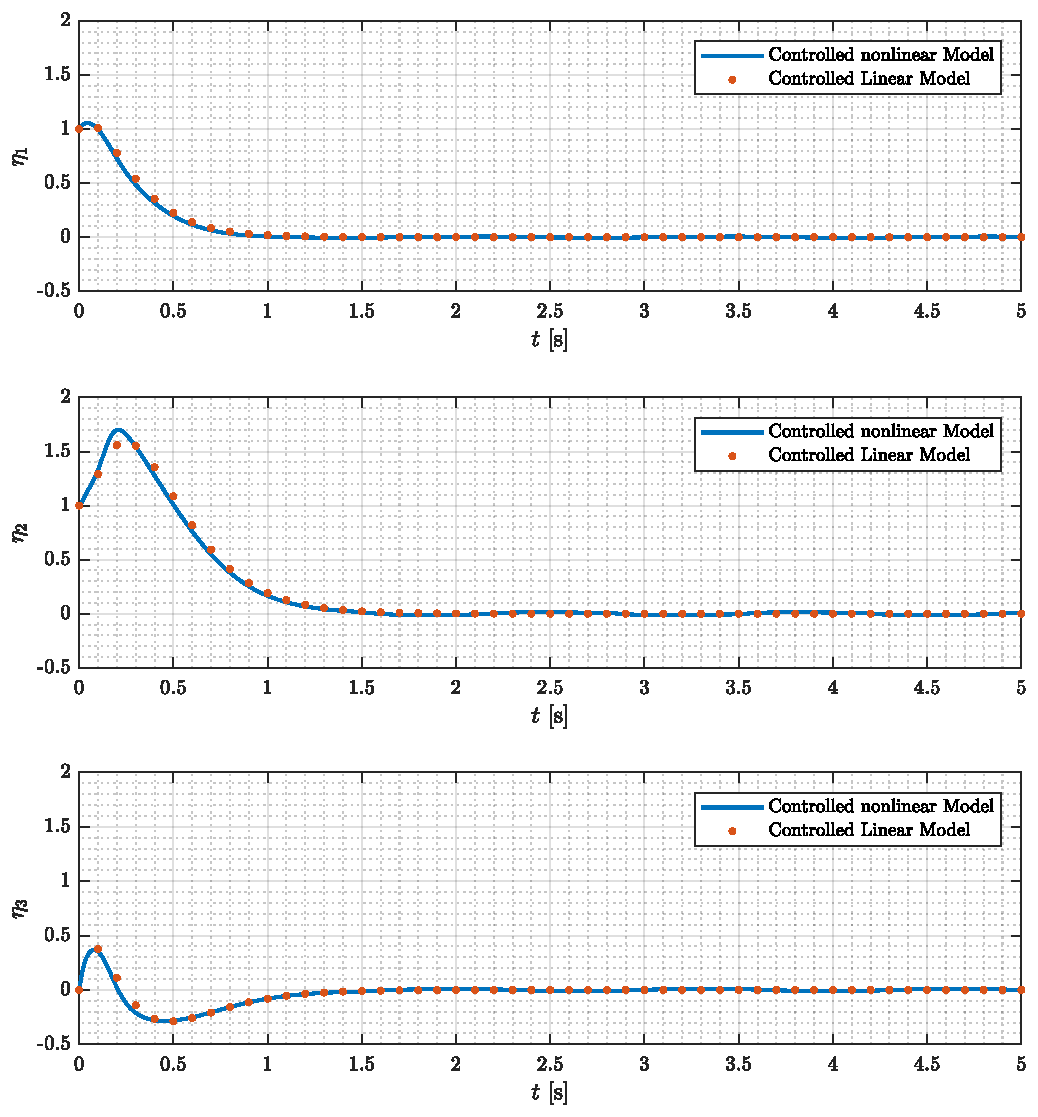
\includegraphics[width=\textwidth]{figures/reducedOrderControl}
    \end{figure}
  \end{minipage}
\end{minipage}
\end{frame}

\begin{frame}{Nonlinear Control}{Sliding Mode}
  \small
  %
  $V = \frac{1}{2}s^2$
  %
  \begin{flalign}
    \dot{V} &= s\dot{s} & \nonumber \\
    \dot{V} &= s ( \dot{\xi} + \vec{k}\dot{\vec{\eta}}  ) & \nonumber \\
    %\dot{V} &= s ( f_b(\vec{\eta},\xi) + g_b(\vec{\eta},\xi) F +\vec{k}f_a(\vec{\eta},\xi) )  & \nonumber \\
    %\dot{V} &= ( \vec{k}f_a(\vec{\eta},\xi)  +  f_b(\vec{\eta},\xi) )s + g_b(\vec{\eta},\xi) s F  & \nonumber \\
    \dot{V} &= g_b(\vec{\eta},\xi) s (\vec{k}f_a(\vec{\eta},\xi)  +  f_b(\vec{\eta},\xi)) g_b^{-1}(\vec{\eta},\xi) + g_b(\vec{\eta},\xi) s F  & \nonumber  \\
    \dot{V} &\leq g_b(\vec{\eta},\xi) |s| \left|\vec{k}f_a(\vec{\eta},\xi) g_b^{-1}(\vec{\eta},\xi) +  f_b(\vec{\eta},\xi) \right| + g_b(\vec{\eta},\xi) s F  \nonumber & \\
    \dot{V} &\leq g_b(\vec{\eta},\xi) |s| \left|\vec{k}f_a(\vec{\eta},\xi) +  f_b(\vec{\eta},\xi) \right|  g_b^{-1}(\vec{\eta},\xi)  & \nonumber \nonumber \\
    &- g_b(\vec{\eta},\xi) \text{sgn}(s) s \left|\vec{k}f_a(\vec{\eta},\xi)  +  f_b(\vec{\eta},\xi) \right| g_b^{-1}(\vec{\eta},\xi)  & \nonumber
  \end{flalign}
  \begin{flalign}
    F &= -\text{sgn}(s)\varrho(\vec{\eta},\xi) g_b^{-1}(\vec{\eta},\xi) \ \ \ \ \text{where}, \ \ \ \varrho(\vec{\eta},\xi)  \geq \left|\vec{k}f_a(\vec{\eta},\xi)  +  f_b(\vec{\eta},\xi) \right|  \nonumber &
  \end{flalign}
  %\begin{flalign}
  %F &= -\text{sgn}(s)\beta (\vec{\eta},\xi) g_b^{-1}(\vec{\eta},\xi) \ \ \ \ \text{where}, \ \ \ \beta(\vec{\eta},\xi) = \varrho(\vec{\eta},\xi) + \beta_0  & \nonumber
  %\normalsize
  %\end{flalign}
  \begin{flalign}
    F &= -\text{sat}(\tfrac{s}{\varepsilon})\beta (\vec{\eta},\xi)  g_b^{-1}(\vec{\eta},\xi) \ \ \ \ \text{where}, \ \ \ \beta(\vec{\eta},\xi) = \varrho(\vec{\eta},\xi) + \beta_0   & \nonumber
  \end{flalign}
  \normalsize
\end{frame}

\begin{frame}{Nonlinear Control}{Sliding Mode}
\small
  \begin{figure}[H]
    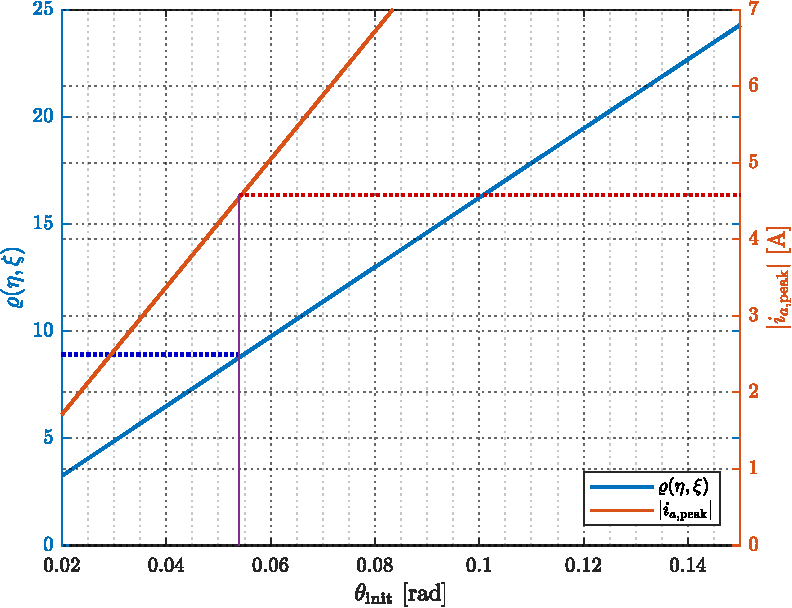
\includegraphics[width=.75\textwidth]{figures/chooseRho}
  \end{figure}
\normalsize
\end{frame}


%-------Nonlinear Control-----(Simulation)--------------------------------

\begin{frame}{Nonlinear Control}{Simulation}
  \hspace{-.9cm}
  \begin{minipage}{\textwidth}
    \begin{minipage}{0.56\textwidth}
      \begin{figure}[H]
        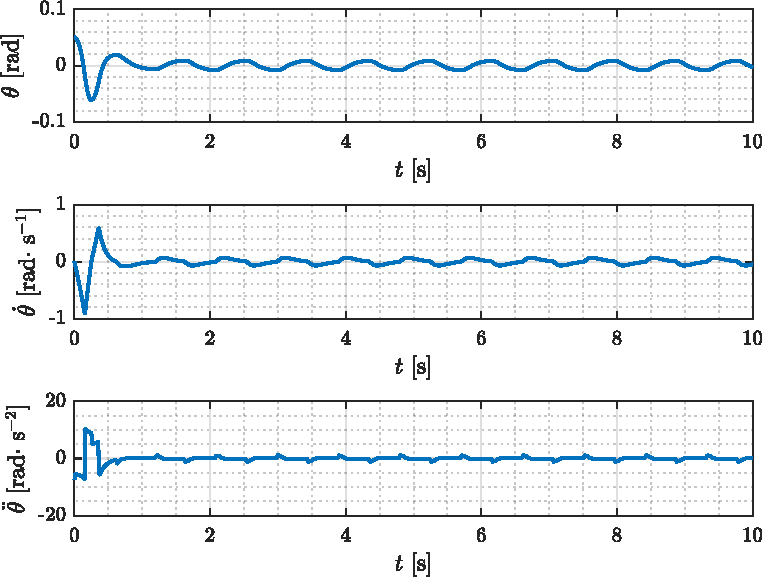
\includegraphics[width=\textwidth]{figures/slidingModeSIMtheta}
      \end{figure}
    \end{minipage}
    \begin{minipage}{0.56\textwidth}
      \begin{figure}[H]
        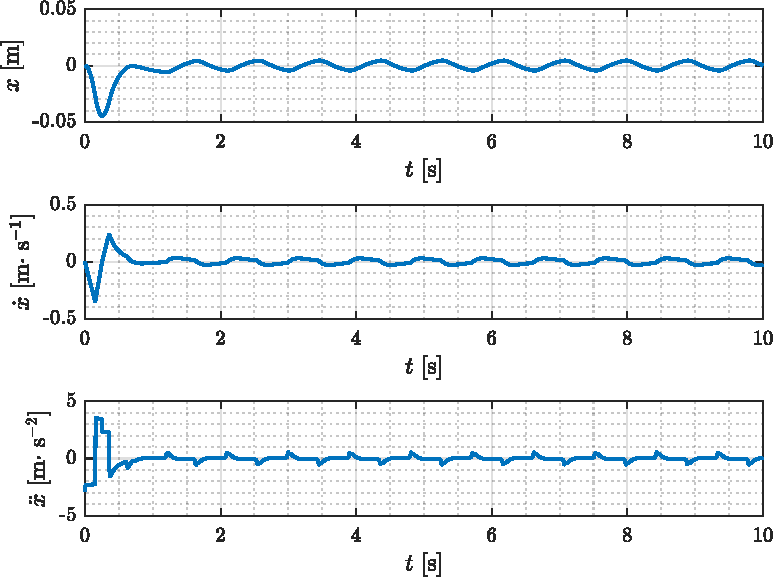
\includegraphics[width=\textwidth]{figures/slidingModeSIMx}
      \end{figure}
    \end{minipage}
  \end{minipage}
\end{frame}

\begin{frame}{Nonlinear Control}{Simulation}
\begin{figure}[H]
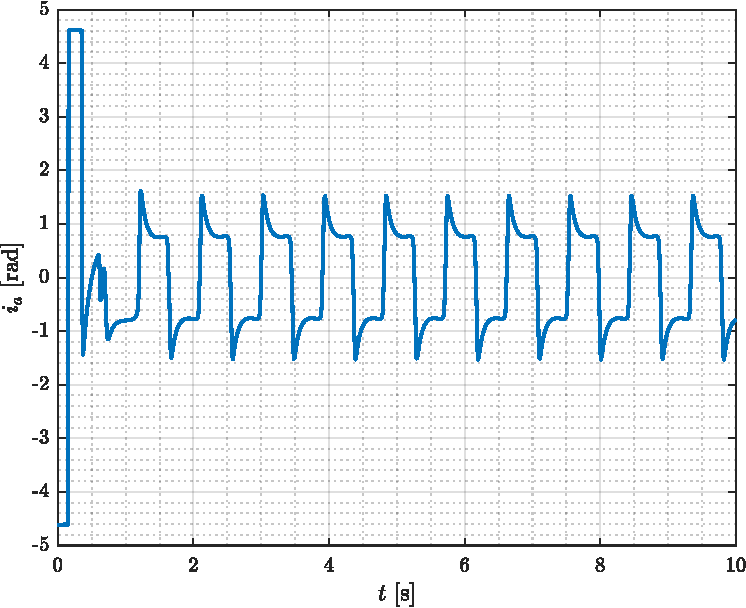
\includegraphics[width=.7\textwidth]{figures/slidingModeSIMia}
\end{figure}
\end{frame}


%-------Trajectory Planning--------------------------------------------------

\begin{frame}{Trajectory Planning}{System}
  \small
  \vspace{-.5cm}
  \begin{figure}[H]
    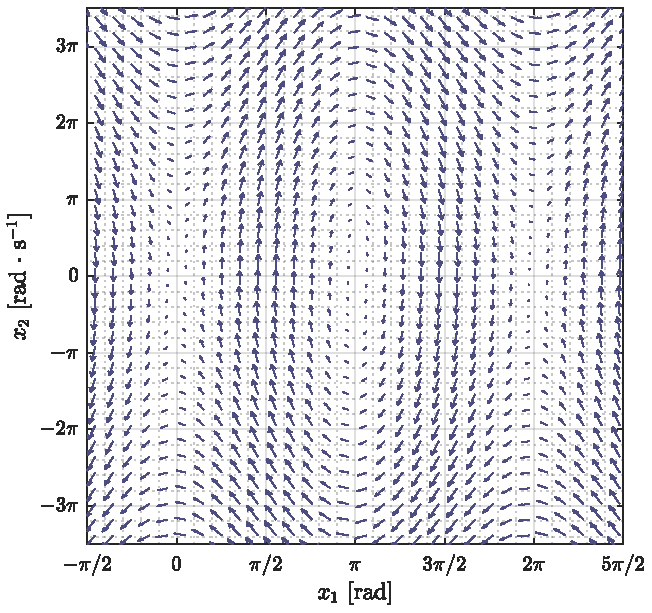
\includegraphics[width=.6\textwidth]{figures/modelPhasePlot}
  \end{figure}
  \vspace{-.5cm}
  \begin{flalign}
    \begin{cases}
    m l^2 \ddot{\theta} - m l \cos \theta \ddot{x} - m g l \sin \theta  = 0  & \nonumber \\   
    ( M + m )\ddot{x} + m l \sin \theta \dot{\theta}^2 - m l \cos \theta \ddot{\theta}  =  F   &  
    \end{cases} && \nonumber
  \end{flalign}
\normalsize
\end{frame}

\begin{frame}{Trajectory Planning}{Integral of System}
\small
  \vspace{-.5cm}
  \begin{flalign}
    \underbrace{ \left( m l^2 - \frac{m^2 l^2}{M + m} \cos^2 \theta \right)    }_{\alpha(\theta)}
    \ddot{\theta} +
    \underbrace{ \left( \frac{m^2 l^2}{M + m} \cos \theta \sin \theta \right)  }_{\beta(\theta)}
    \dot{\theta}^2
    \underbrace{ - m g l \sin \theta - \frac{m l}{M + m} \cos \theta F         }_{\gamma(\theta)}
    &=  0    && \nonumber
  \end{flalign}
  \begin{flalign}
  \alpha (\theta) \ddot{\theta} + \beta (\theta) \dot{\theta}^2 + \gamma (\theta) &=  0   \nonumber & 
  \end{flalign}
  %
  \begin{flalign}
  I(\theta,\dot{\theta},\theta_0,\dot{\theta}_0) &=
   \int \alpha (\theta) \ddot{\theta} + \beta (\theta) \dot{\theta}^2 + \gamma (\theta)\ d\theta   \nonumber &  
  \end{flalign}
  %
  \begin{flalign}
    I(\theta,\dot{\theta},\theta_0,\dot{\theta}_0) &=
    \dot{\theta}^2 -
    \text{exp}
    \left[ 
    -2 \int\limits_{\theta_0}^{\theta} \frac{\beta(\tau)}{\alpha(\tau)} d\tau
    \right]
    \left(
    \dot{\theta}_0^2 -
    \int\limits_{\theta_0}^{\theta}
    \text{exp}
    \left[
    2 \int\limits_{\theta_0}^{s} \frac{\beta(\tau)}{\alpha(\tau)} d\tau
    \right]
    \frac{2 \gamma (s)}{\alpha (s)}
    ds
    \right)  \nonumber &  
  \end{flalign}
\normalsize
\end{frame}

\begin{frame}{Trajectory Planning}{Trajectories}
  \small
  \vspace{-.25cm}
  \begin{flalign}
    I(\theta,\dot{\theta},\theta_0,\dot{\theta}_0) &=
    \dot{\theta}^2 -
    \text{exp}
    \left[ 
    -2 \int\limits_{\theta_0}^{\theta} \frac{\beta(\tau)}{\alpha(\tau)} d\tau
    \right]
    \left(
    \dot{\theta}_0^2 -
    \int\limits_{\theta_0}^{\theta}
    \text{exp}
    \left[
    2 \int\limits_{\theta_0}^{s} \frac{\beta(\tau)}{\alpha(\tau)} d\tau
    \right]
    \frac{2 \gamma (s)}{\alpha (s)}
    ds
    \right)  \nonumber &  
  \end{flalign}
  \begin{figure}[H]
    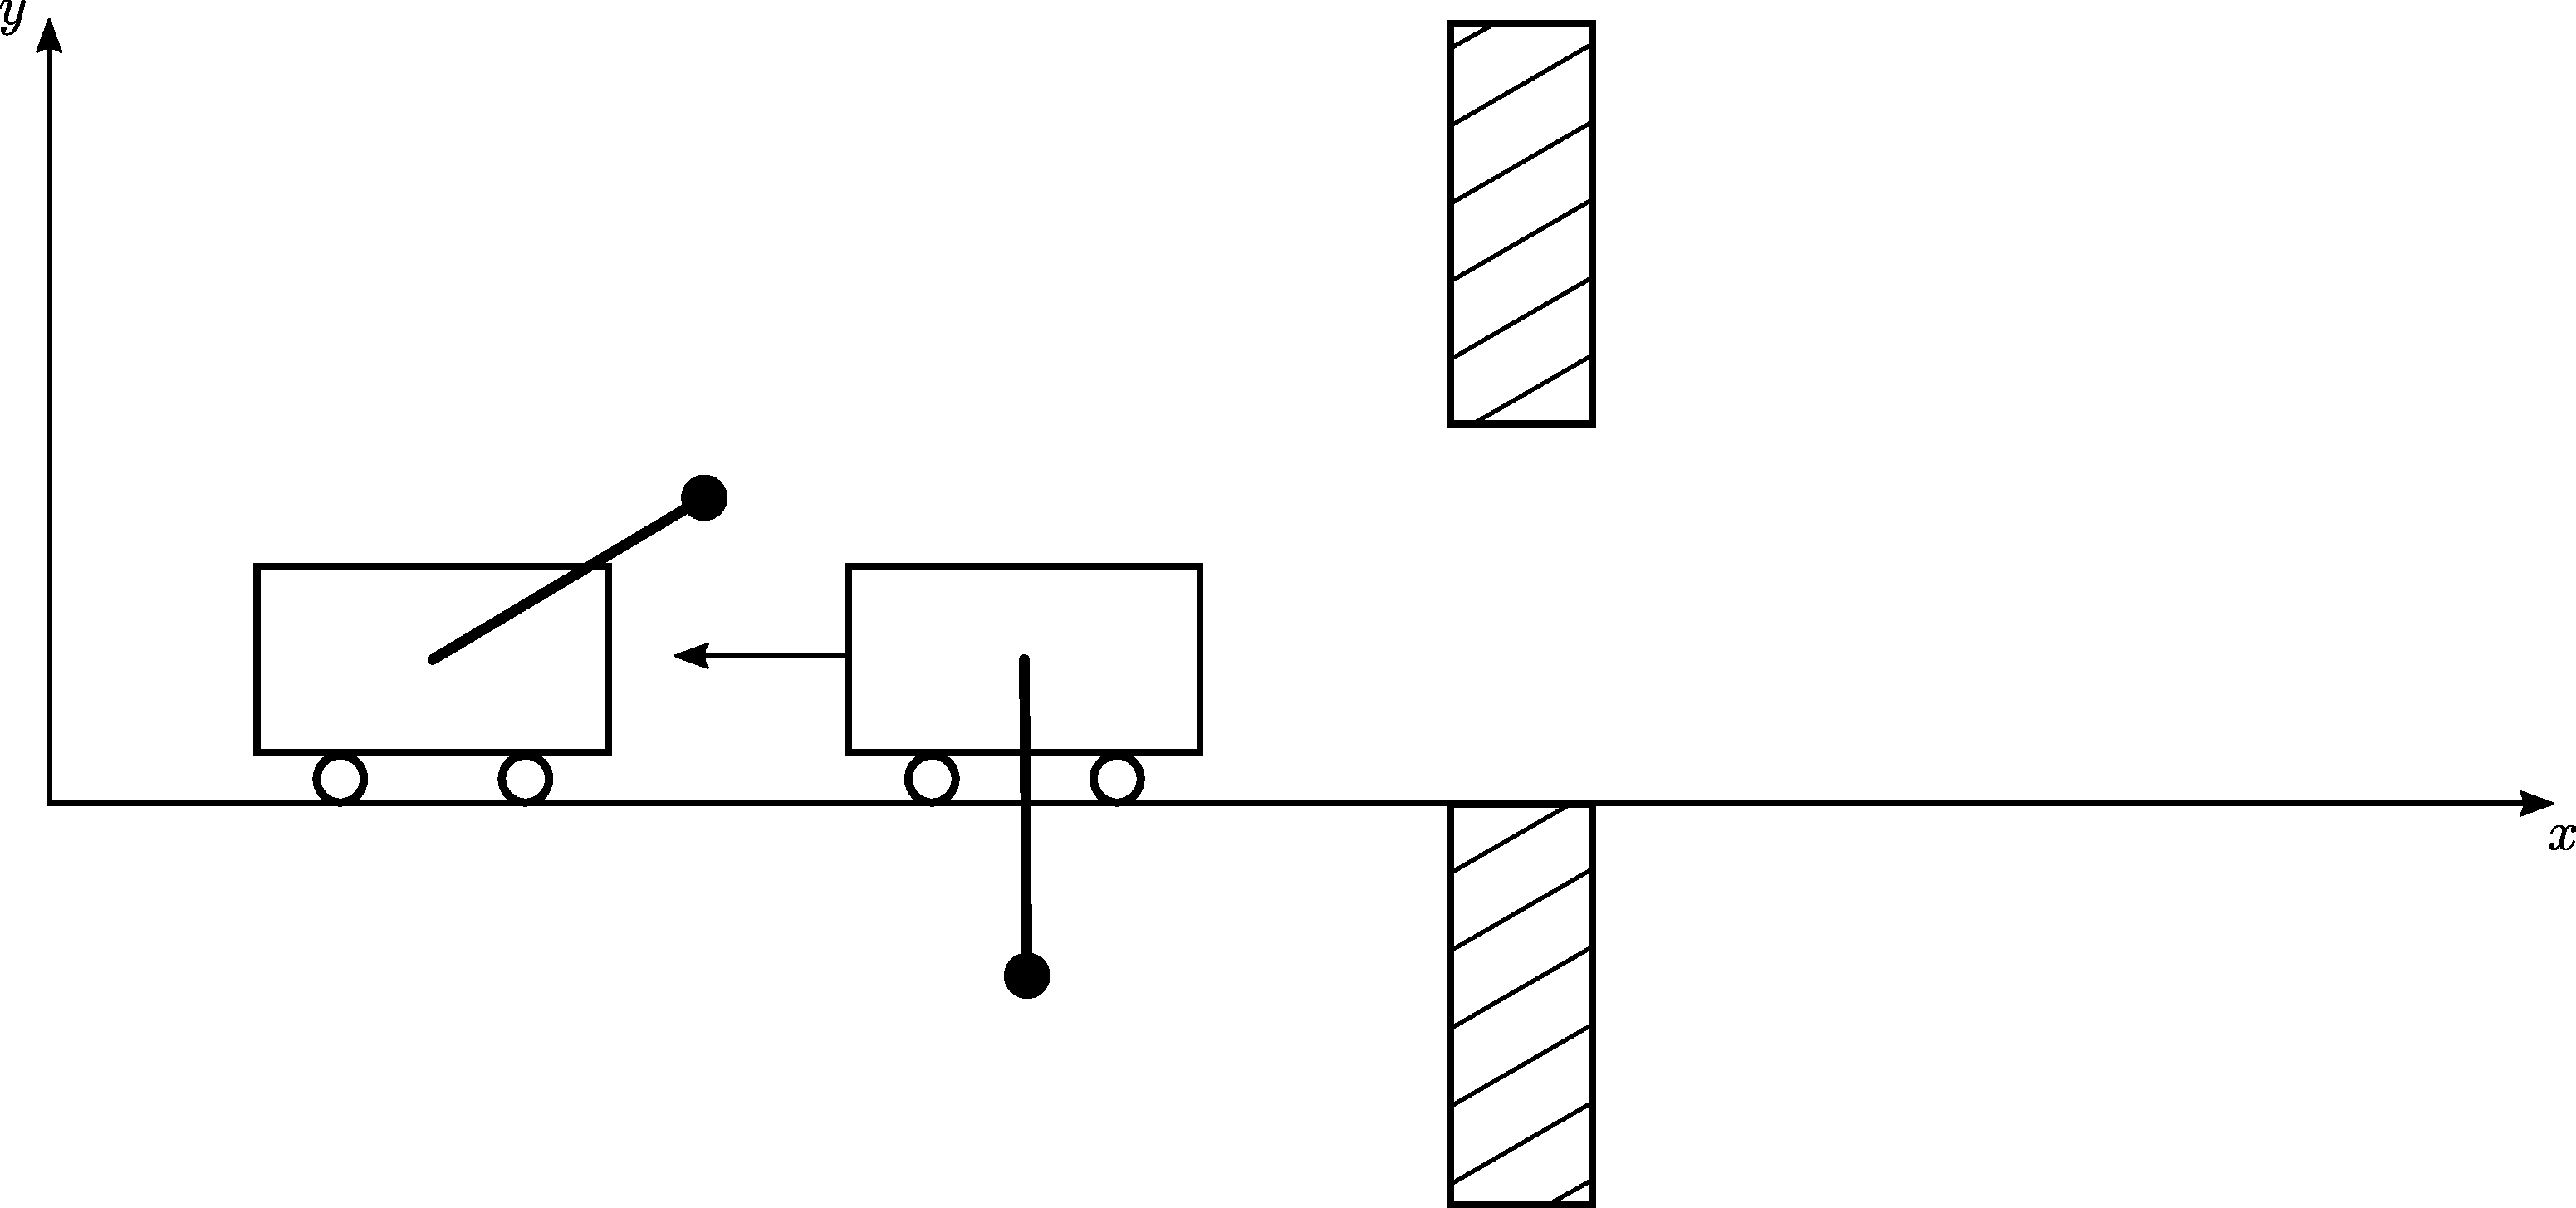
\includegraphics[width=.7\textwidth]{figures/firstTask}
  \end{figure}
  \begin{flalign}
    I(\theta,\dot{\theta},\theta_0,\dot{\theta}_0) &= \frac{m l^2 - \frac{m^2 l^2}{M + m}}{m l^2 - \frac{m^2 l^2}{M + m} \cos^2 \theta}
    \left(
    - 4 \left[ \frac{ M g + m g - F \tan\frac{s}{2} }{M l (\tan^2\frac{s}{2} + 1)}  \right]_{\theta_0}^\theta
    \right) & \nonumber
  \end{flalign}
  \normalsize
\end{frame}

\begin{frame}{Trajectory Planning}{Solution}
  \small
  \vspace{-.5cm}
  \begin{flalign}
    \begin{cases}
      m l^2 \ddot{\theta} - m l \cos \theta \ddot{x} - m g l \sin \theta  = 0  & \nonumber \\   
      ( M + m )\ddot{x} + m l \sin \theta \dot{\theta}^2 - m l \cos \theta \ddot{\theta}  =  F   &  
    \end{cases} && \nonumber
  \end{flalign}
  \begin{figure}[H]
    \includegraphics[width=.7\textwidth]{figures/secondTask}
  \end{figure}
  \vspace{-1cm}
  \begin{flalign}
  \begin{cases}
  - m l \cos \theta \ddot{x} - m g l \sin \theta  = 0  & \\
  ( M + m )\ddot{x}  =  F 
  \end{cases} \nonumber &&
  \end{flalign}
  \normalsize
\end{frame}


%-------Results-----(Sliding Mode)----------------------------------------

\begin{frame}{Results}{Sliding Mode}
\hspace{-.9cm}
\begin{minipage}{\textwidth}
  \begin{minipage}{0.56\textwidth}
    \begin{figure}[H]
      \includegraphics[width=\textwidth]{figures/slidingModeTest2theta}
    \end{figure}
  \end{minipage}
  \begin{minipage}{0.56\textwidth}
    \begin{figure}[H]
      \includegraphics[width=\textwidth]{figures/slidingModeTest2x}
    \end{figure}
  \end{minipage}
\end{minipage}
\end{frame}

\begin{frame}{Results}{Sliding Mode}
\begin{figure}[H]
  \includegraphics[width=.7\textwidth]{figures/slidingModeTest2ia}
\end{figure}
\end{frame}

%-------Results-----(Trajectory Planning)--------------------------------
  
\begin{frame}{Results}{Trajectory Planning}
\begin{figure}[H]
  \includegraphics[width=.6\textwidth]{figures/firstTraj}
\end{figure}
\end{frame}

\begin{frame}{Results}{Trajectory Planning}
\begin{figure}[H]
  \includegraphics[width=.6\textwidth]{figures/thirdTraj}
\end{figure}
\end{frame}

\begin{frame}{Results}{Trajectory Planning}
\hspace{-1cm}
\begin{minipage}{1\textwidth}
  \begin{figure}[H]
    \includegraphics[width=1.15\textwidth]{figures/trajectoryAnimation}
  \end{figure}
\end{minipage}
\end{frame}

%\definecolor{aaublue}{RGB}{33,26,82}% dark blue

\begin{frame}<handout:0>{Agenda}{}
    \begin{itemize}
        \item Introduction
        \item System Description
        \item Model
        \item Control Approach
        \item Sensor Fusion
        \item \textcolor{aaublue}{\textbf{Inner Controller}}
        \begin{itemize}
            \item[-] $\mathcal{H}_\infty$ Controller Design
            \item[-] \textcolor{aaublue}{\textbf{Linear Quadratic Regulator Design}}
            \item[-] \textcolor{aaublue}{\textbf{Controllers Comparison}}
        \end{itemize}
        \item Outer Controller
        \item Results
        \item Conclusion
    \end{itemize}
\end{frame}
%\begin{frame}{Introduction}{The System}

\begin{figure}[H]
  \includegraphics[width=.2\textwidth]{figures/system}
\end{figure}














%\only<1| handout:0>
%{
%  %\item Discrete system representation
%
%  \tikz[overlay,xshift=15em,yshift=1em]{\draw node {
%      \begin{minipage}{0.8\linewidth}
%        \begin{figure}[H]
%          \includegraphics[width=1\textwidth]{figures/LQRblockDiagram1}
%        \end{figure}
%      \end{minipage}
%    };}
%  
%  
%  \tikz[overlay,xshift=12em,yshift=-5em]{\draw node {
%      \begin{minipage}{0.01\linewidth}
%        \begin{flalign}
%          \vec{x}(k+1) &= \vec{A}_z  \vec{x}(k) + \vec{B}_z  \vec{u}(k) \nonumber \\
%          \vec{y}(k) &= \vec{C}_z x(k) + \vec{D}_z  \vec{u}(k) \nonumber
%        \end{flalign}
%      \end{minipage}
%  };}
%  
%}

\uncover<1-2>
{
  %\item Adding a reference
  %\tikz[overlay,xshift=15em,yshift=1em]{\draw node {
    %\begin{minipage}{0.8\linewidth}
      \begin{figure}[H]
        \includegraphics[width=1\textwidth]{figures/system}
      \end{figure}
    %\end{minipage}
  %};}
}

%\only<0| handout:1>
%{
%  \tikz[overlay,xshift=12em,yshift=-2.5em]{\draw node {
%      \begin{minipage}{0.01\linewidth}
%        \begin{flalign}
%        \vec{x}(k+1) &= \vec{A}_z  \vec{x}(k) + \vec{B}_z  \vec{u}(k) \nonumber \\
%        \vec{y}(k) &= \vec{C}_z x(k) + \vec{D}_z  \vec{u}(k) \nonumber
%        \end{flalign}
%      \end{minipage}
%    };}
%}

%\only<2| handout:0>
%{
%  \tikz[overlay,xshift=12em,yshift=-5.5em]{\draw node {
%  };}
%}

%\only<3| handout:0>
%{
%  \tikz[overlay,xshift=12em,yshift=-5em]{\draw node {
%    \begin{minipage}{0.01\linewidth}
%      \begin{flalign}
%        \vec{x}_e(k+1) &= \vec{A}_e  \vec{x}_e(k) + \vec{B}_e  \vec{u}(k) + \vec{r}(k) \nonumber \\
%        \vec{y}(k) &= \vec{C}_e  \vec{x}_e(k) \nonumber
%      \end{flalign}
%    \end{minipage}
%  };}
%}

\uncover<2>
{
  %\tikz[overlay,xshift=12em,yshift=-5.5em]{\draw node {
    %\begin{minipage}{0.01\linewidth}
      \begin{flalign}
     %\hspace{2cm}
        \begin{bmatrix}
          \vec{x}(k+1)  \\
          \vec{x}_\mathrm{I}(k+1)
        \end{bmatrix}
        &=
        \begin{bmatrix}
         \ \ \ \vec{A}_\mathrm{z,3x3} & \vec{0}_\mathrm{3x2} \\
         -\vec{C}_\mathrm{z,2x3} & \vec{I}_\mathrm{2x2} \\
        \end{bmatrix}
        \begin{bmatrix}
          \vec{x}(k)    \\
          \vec{x}_\mathrm{I}(k)
        \end{bmatrix}
        +
        \begin{bmatrix}
          \vec{B}_\mathrm{z,3x2} \\
          \vec{0}_\mathrm{2x2}
        \end{bmatrix}
        \vec{u}(k)
        +
        \begin{bmatrix}
          \vec{0}_\mathrm{3x2} \\
          \vec{I}_\mathrm{2x2}
        \end{bmatrix}
        \vec{r}(k) \nonumber \\ \nonumber \\[-10pt]
        \vec{y}(k)
        &=
        \begin{bmatrix}
          \vec{C}_\mathrm{z,2x3} &  \vec{0}_\mathrm{2x2}
        \end{bmatrix}
        \begin{bmatrix}
          \vec{x}(k)    \\
          \vec{x}_\mathrm{I}(k)
        \end{bmatrix} \nonumber
      \end{flalign}
    %\end{minipage}
  %};}
}

\end{frame}

\begin{frame}{Inner Controller}{Linear Quadratic Controller Design}
\only<1| handout:0>
{   
  \tikz[overlay,xshift=12em,yshift=3em]{\draw node {
    \begin{minipage}{0.8\linewidth}    
          \begin{itemize}
              \item Discrete cost function
            \end{itemize}    
      \begin{flalign}
      \mathcal{J}_\mathrm{z} = \sum_{k=0}^\infty \vec{x}^\mathrm{T}(k)\vec{Q}_\mathrm{z}\vec{x}(k) + \vec{u}^\mathrm{T}(k)\vec{R}_\mathrm{z}\vec{u}(k) \nonumber
      \end{flalign}
    \end{minipage}
  };}
  \tikz[overlay,xshift=12em,yshift=-.5em]{\draw node {
  };}
  \tikz[overlay,xshift=12em,yshift=-5em]{\draw node {
  };}
}

\only<2-3| handout:1>
{
  \tikz[overlay,xshift=12em,yshift=3em]{\draw node {
      \begin{minipage}{0.8\linewidth}
          \begin{itemize}
              \item Continuous cost function
           \end{itemize}
        \begin{flalign}
        \hspace{-.7cm}
        \mathcal{J}= \int_{0}^\infty \vec{x}^\mathrm{T}(t)\vec{Q}\vec{x}(t) + \vec{u}^\mathrm{T}(t)\vec{R}\vec{u}(t) \ dt \nonumber
        \end{flalign}
      \end{minipage}
    };}
  \tikz[overlay,xshift=12em,yshift=-.5em]{\draw node {
    };}
  \tikz[overlay,xshift=12em,yshift=-5em]{\draw node {
    };}
}


\only<1-2| handout:0>
{
  \tikz[overlay,xshift=12em,yshift=-.5em]{\draw node {
  };}
}

\only<3| handout:1>
{
  \tikz[overlay,xshift=12em,yshift=-1.6em]{\draw node {
    \begin{minipage}{0.8\linewidth}
      \begin{flalign} 
        \hspace{3cm}
        Q &= diag\left(
        \frac{1}{{\psi_\mathrm{max}}\text{}^2} \ , \ 
        \frac{1}{{\dot{\psi}_\mathrm{max}}\text{}^2} \ , \ 
        \frac{1}{{\dot{x}_{b,\mathrm{max}}}\text{}^2} \ , \ 
        \frac{1}{x_{\mathrm{I},\psi,\mathrm{max}}\text{}^2} \ , \
        \frac{1}{x_{\mathrm{I},\dot{x_b},\mathrm{max}}\text{}^2} \right)
        \nonumber
      \end{flalign}
%      \begin{flalign}
%      \dot{\vec{x}}(t) &= \vec{A}  \vec{x}(t) + \vec{B}  \vec{u}(t) + r(t)\nonumber \\
%      \vec{y}(t) &= \vec{C} x(t)  \nonumber
%      \end{flalign}
    \end{minipage}
  };}
}

\only<1-2| handout:0>
{
  \tikz[overlay,xshift=12em,yshift=-5em]{\draw node {
  };}
}

\only<3| handout:1>
{
  \tikz[overlay,xshift=12em,yshift=-5em]{\draw node {
  \begin{minipage}{0.8\linewidth}
    \begin{flalign}
      \hspace{-1cm}
      R &= diag\left(
      \frac{1}{{{F_1}_\mathrm{max}}\text{}^2} \ , \ 
      \frac{1}{{{F_2}_\mathrm{max}}\text{}^2} \right)
      \nonumber
    \end{flalign}
%    \begin{flalign}
%      \hspace{2cm}
%      \begin{bmatrix}
%        \dot{\vec{x}}(t)  \\
%        \dot{\vec{x}}_\mathrm{I}(t)
%      \end{bmatrix}
%      &=
%      \begin{bmatrix}
%      \ \ \ \vec{A}_\mathrm{3x3} & \vec{0}_\mathrm{3x2} \\
%       -\vec{C}_\mathrm{2x3} & \vec{I}_\mathrm{2x2} \\
%      \end{bmatrix}
%      \begin{bmatrix}
%        \vec{x}(t)    \\
%        \vec{x}_\mathrm{I}(t)
%      \end{bmatrix}
%      +
%      \begin{bmatrix}
%        \vec{B}_\mathrm{3x2} \\
%        \vec{0}_\mathrm{2x2}
%      \end{bmatrix}
%      \vec{u}(k)
%      +
%      \begin{bmatrix}
%        \vec{0}_\mathrm{3x2} \\
%        \vec{I}_\mathrm{2x2}
%      \end{bmatrix}
%      \vec{r}(t) \nonumber \\ \nonumber \\[-10pt]
%      \vec{y}(t)
%      &=
%      \begin{bmatrix}
%        \vec{C}_\mathrm{2x3} &  \vec{0}_\mathrm{2x2}
%      \end{bmatrix}
%      \begin{bmatrix}
%        \vec{x}(t)    \\
%        \vec{x}_\mathrm{I}(t)
%      \end{bmatrix} \nonumber
%    \end{flalign}
  \end{minipage}
  };}
}
\end{frame}

\begin{frame}{Inner Controller}{Linear Quadratic Controller Design}
    \begin{itemize}
        \item Discretize the cost function to get $\vec{Q}_z$ and $\vec{R}_z$
        \vspace{.3cm}
        \item Solve the discrete-time algebraic Riccati equation
        \vspace{.3cm}
        \item Get the feedback gains
    \end{itemize}
        \vspace{.5cm}
    \begin{flalign}
        \hspace{-2cm}
        \vec{u}(k) = - 
        \begin{bmatrix}
            \vec{F} & \vec{F}_\mathrm{I}
            \end{bmatrix}
            \begin{bmatrix}
            \vec{x}(k)  \\
            \vec{x}_\mathrm{I}(k)
        \end{bmatrix} \nonumber
    \end{flalign}
\end{frame}

\begin{frame}{Inner Controller}{Comparison of the Controllers}
  \textbf{Simulation of LQR and $\mathcal{H}_\infty$ design}
  \vspace{.2cm}
  \begin{itemize}
    \item<1-> Wind and current disturbances
    \begin{itemize}
      \item<1-> $\pm 1.5$ N along $\dot{x}_b$
      \item<1-> $\pm 1.5$ N$\cdot$m around $z_b$
    \end{itemize}
    \item<1-> Wave disturbance
    \begin{itemize}
      \item<1-> Sinusoidal
      \item<1-> frequency between $0$-$10$ Hz
    \end{itemize}
    \item<2-> The parameters are varied $\pm 20\%$
    \begin{itemize}
      \item<2-> Mass, $m$
      \item<2-> Moment of inertia, $I_z$, around $z_b$
      \item<2-> The damping coefficients $d_x$ and $d_\psi$
      \item<2-> The lengths $l_1$ and $l_2$
    \end{itemize}
  \item<3-> Monte Carlo simulations with $1000$ realizations
  \end{itemize}
\end{frame}


\begin{frame}{Inner Controller}{Comparison of the Controllers}
\begin{figure}[H]
  \begin{minipage}{0.45\linewidth}
    \begin{figure}[H]
      \centering
      \includegraphics[width=1\linewidth]{figures/xbdot_mc_lqr}
    \end{figure}        
  \end{minipage}\hfill      
  \begin{minipage}{0.45\linewidth}
    \begin{figure}[H]
      \centering
      \includegraphics[width=1\linewidth]{figures/xbdot_mc_rob}
    \end{figure}                
  \end{minipage}\hfill \\
\end{figure}
\begin{itemize}
    \item Influence from change in reference in $\psi$
    \item LQR gives a faster response
    \item $\mathcal{H}_\infty$ controller is more robust to disturbances
\end{itemize}
\end{frame}


\begin{frame}{Inner Controller}{Comparison of the Controllers}
  \begin{figure}[H]
    \begin{minipage}{0.45\linewidth}
      \begin{figure}[H]
        \centering
        \includegraphics[width=1\linewidth]{figures/xbdot_mc_lqr_error}
      \end{figure}        
    \end{minipage}\hfill      
    \begin{minipage}{0.45\linewidth}
      \begin{figure}[H]
        \centering
        \includegraphics[width=1\linewidth]{figures/xbdot_mc_rob_error}
      \end{figure}                
    \end{minipage}\hfill \\
  \end{figure}
\begin{itemize}
  \item Influence from change in reference in $\psi$
  \item LQR gives a faster response
  \item $\mathcal{H}_\infty$ controller is more robust to disturbances
\end{itemize}
\end{frame}



\begin{frame}{Inner Controller}{Comparison of the Controllers}
  \begin{figure}[H]
    \begin{minipage}{0.45\linewidth}
      \begin{figure}[H]
        \centering
        \includegraphics[width=1\linewidth]{figures/yaw_mc_lqr}
      \end{figure}        
    \end{minipage}\hfill      
    \begin{minipage}{0.45\linewidth}
      \begin{figure}[H]
        \centering
        \includegraphics[width=1\linewidth]{figures/yaw_mc_rob}
      \end{figure}                
    \end{minipage}\hfill \\
  \end{figure}
    \begin{itemize}
        \item LQR gives a faster response
        \item $\mathcal{H}_\infty$ controller is more robust to disturbances
        \item $\mathcal{H}_\infty$ controller tracks $\psi$ fast but $\dot{x}_b$ slow
    \end{itemize}
\end{frame}

\begin{frame}{Inner Controller}{Comparison of the Controllers}
  \begin{figure}[H]
    \begin{minipage}{0.45\linewidth}
      \begin{figure}[H]
        \centering
        \includegraphics[width=1\linewidth]{figures/yaw_mc_lqr_error}
      \end{figure}        
    \end{minipage}\hfill      
    \begin{minipage}{0.45\linewidth}
      \begin{figure}[H]
        \centering
        \includegraphics[width=1\linewidth]{figures/yaw_mc_rob_error}
      \end{figure}                
    \end{minipage}\hfill \\
  \end{figure}
    \begin{itemize}
      \item LQR gives a faster response
      \item $\mathcal{H}_\infty$ controller is more robust to disturbances
      \item $\mathcal{H}_\infty$ controller tracks $\psi$ fast but $\dot{x}_b$ slow
    \end{itemize}
\end{frame}



%\definecolor{aaublue}{RGB}{33,26,82}% dark blue

\begin{frame}<handout:0>{Agenda}{}
    \begin{itemize}
        \item Introduction
        \item System Description
        \item Model
        \item Control Approach
        \item Sensor Fusion
        \item Inner Controller
        \item \textcolor{aaublue}{\textbf{Outer Controller}}
        \begin{itemize}
            \item[-] \textcolor{aaublue}{\textbf{Path Generation Algorithm}}
            \item[-] \textcolor{aaublue}{\textbf{Path Following Algorithm}}
        \end{itemize}
        \item \textcolor{aaublue}{\textbf{Results}}
        \begin{itemize}
            \item[-] \textcolor{aaublue}{\textbf{Controller Results}}
            \item[-] \textcolor{aaublue}{\textbf{Implementation Results}}
        \end{itemize}
        \item \textcolor{aaublue}{\textbf{Conclusion}}
    \end{itemize}
\end{frame}
%%%%%%%%%%%%%%%%%
\section{Outer Controller}

\begin{frame}{Outer Controller}{Path Generation Algorithm}
    \begin{figure}[H]
        \centering
        \includegraphics[width=1\textwidth]{figures/pathGen} 
    \end{figure}       
\end{frame}

\begin{frame}{Outer Controller}{Path Following Algorithm}
    \begin{minipage}{0.6\linewidth}
        \uncover<1-4>{
        \begin{figure}[H]
            \centering
            \includegraphics[width=0.9\linewidth]{figures/LOSalgorithm}
        \end{figure} }       
    \end{minipage}\hfill      
    \begin{minipage}{0.2\linewidth}
        \uncover<2-4>{
        \begin{flalign}
            \chi &= \arctan\left(\frac{y_\mathrm{LOS}-y_\mathrm{n}}{x_\mathrm{LOS}-x_\mathrm{n}}\right)\nonumber 
        \end{flalign} }
        \uncover<3-4>{
        \begin{flalign}
            \beta &= \arctan\left(\frac{\dot{y}_\mathrm{b}}{\dot{x}_\mathrm{b}}\right) \nonumber
        \end{flalign} }
        \uncover<4>{
        \begin{flalign}
            \psi&_\mathrm{ref} = \chi - \beta \nonumber
        \end{flalign}}          
    \end{minipage}\hfill \\ 
\end{frame}

\begin{frame}{Outer Controller}{Path Following Algorithm}
    \begin{itemize}
        \item Change active waypoints
    \end{itemize}
    \begin{figure}[H]
        \centering
        \includegraphics[width=0.6\linewidth]{figures/LOSalgorithmdistancewp}
    \end{figure}
\end{frame}
\begin{frame}{Outer Controller}{Path Following Algorithm}
    \begin{itemize}
        \item Convergence to the path
    \end{itemize}
    \begin{minipage}{0.45\linewidth}
        \begin{figure}[H]
            \centering
            \includegraphics[width=1\linewidth]{figures/patherror}
        \end{figure}     
    \end{minipage}\hfill      
    \begin{minipage}{0.45\linewidth}
        \begin{figure}[H]
            \centering
            \includegraphics[width=1\linewidth]{figures/initCondOuter}
        \end{figure}               
    \end{minipage}\hfill \\
\end{frame}
%%%%%%%%%%%%%%%%
\section{Results}

\begin{frame}{Results}{Controller Results}
\begin{itemize}
    \item LQR as inner controller
\end{itemize}
    \begin{minipage}{0.45\linewidth}
            \begin{figure}[H]
                \centering
                \includegraphics[width=1\linewidth]{figures/path_lqr}
            \end{figure}        
        \end{minipage}\hfill      
    \begin{minipage}{0.45\linewidth}
            \begin{figure}[H]
                \centering
                \includegraphics[width=1\linewidth]{figures/dist_lqr}
            \end{figure}               
        \end{minipage}\hfill \\    
\end{frame}

\begin{frame}{Results}{Controller Results}
    \begin{itemize}
        \item Robust controller as inner controller
    \end{itemize}
    \begin{minipage}{0.45\linewidth}
            \begin{figure}[H]
                \centering
                \includegraphics[width=1\linewidth]{figures/path_rob}
            \end{figure}       
        \end{minipage}\hfill      
    \begin{minipage}{0.45\linewidth}
            \begin{figure}[H]
                \centering
                \includegraphics[width=1\linewidth]{figures/dist_rob}
            \end{figure}             
        \end{minipage}\hfill \\    
\end{frame}

%\begin{frame}{Results}{Implementation Results}
%    \begin{itemize}
%        \item Implementation diagram in ROS
%    \end{itemize}
%    \begin{figure}[H]
%        \centering
%        \includegraphics[width=1\textwidth]{figures/diagramROS}
%    \end{figure}  
%\end{frame}


\begin{frame}{Results}{Implementation Results}
    \begin{itemize}
        \item Inner controller test
    \end{itemize}
    \begin{minipage}{0.45\linewidth}
        \begin{figure}[H]
            \centering
            \includegraphics[width=1\linewidth]{figures/inner_yaw}
        \end{figure}       
    \end{minipage}\hfill      
    \begin{minipage}{0.45\linewidth}
        \begin{figure}[H]
            \centering
            \includegraphics[width=1\linewidth]{figures/inner_xbdot}
        \end{figure}             
    \end{minipage}\hfill \\    
\end{frame}

\begin{frame}{Results}{Implementation Results}
    \begin{itemize}
        \item Actuator tests
    \end{itemize}
    \begin{minipage}{0.45\linewidth}
        \begin{figure}[H]
            \centering
            \includegraphics[width=1\linewidth]{figures/direction}
        \end{figure}       
    \end{minipage}\hfill      
    \begin{minipage}{0.45\linewidth}
        \begin{figure}[H]
            \centering
            \includegraphics[width=1\linewidth]{figures/hysteresis}
        \end{figure}             
    \end{minipage}\hfill \\    
\end{frame}

%%%%%%%%%%%%%%%%
\section{Conclusion}

\begin{frame}{Conclusion}{}
    \begin{itemize}
        \item A dynamic model of the system has been derived
    \end{itemize}
    \begin{itemize}
        \item The estimator has been designed and tested through simulation
    \end{itemize}
    \begin{itemize}
        \item The control system has also been analyzed through simulations that include disturbances, noise and varying parameters
    \end{itemize}
    \begin{itemize}
        \item The simulated results have not been fully replicated in the real vessel, but they show a promising behavior of the control system
    \end{itemize}
\end{frame}

%{\aauwavesbg
\begin{frame}[plain,noframenumbering]
    \finalpage{\large{ Sliding Mode Stabilization and Phase Plane Trajectory Planning for a Cart Pendulum System }}
\end{frame}%}

\end{document}
